\documentclass[a4paper,10pt]{article}
\usepackage[utf8]{inputenc}
\usepackage{graphicx}

%opening
\title{Trafico Automata Nagel-Schreckenberg}
\author{Allan Ulises Zepeda Ibarra}

\begin{document}

\maketitle



\section{Introduccion}

El modelo de Nagel y Schreckenberg (Na-Sch) es un modelo de flujo de tr\'ansito vehicular con un aut\'omata celular. 
El modelo fue desarrollado en la d\'ecada de 1990 por los alemanes f\'\i sicos Kai Nagel y Michael Schreckenberg.
El modelo muestra c\'omo los atascos de tr\'afico pueden ser considerados como un fen\'omeno emergente o colectiva debido a las 
interacciones entre los coches en la carretera, cuando la densidad de veh\'\i culos es alta.

\section{Parametros}

Cada veh\'\i culo tiene asociada una posici\'on x en la autopista.\\
Cada veh\'\i culo tiene una velocidad v asociada, que es un valor entero.\\
Vmax es la m\'axima velocidad que puede alcanzar cualquiera de los veh\'\i culos.\\
P es la probabilidad de que un veh\'\i culo reduzca su velocidad aleatoriamente.\\
b se conoce como la brecha, que es la distancia en c\'elulas que separa a un veh\'\i culo de su predecesor.\\

\subsection{Reglas}

Regla 1.- V=min(v+1,Vmax)
Regla 2.- V=min(v,b)
Regla 3.- p/V=max(v-1,0)
Regla 4.- x=x+v

\section{Desarrollo}

Para este proyecto se aplico el modelo propuesto simulando la carretera con una secuencia de c\'\i rculos.
\\ \\
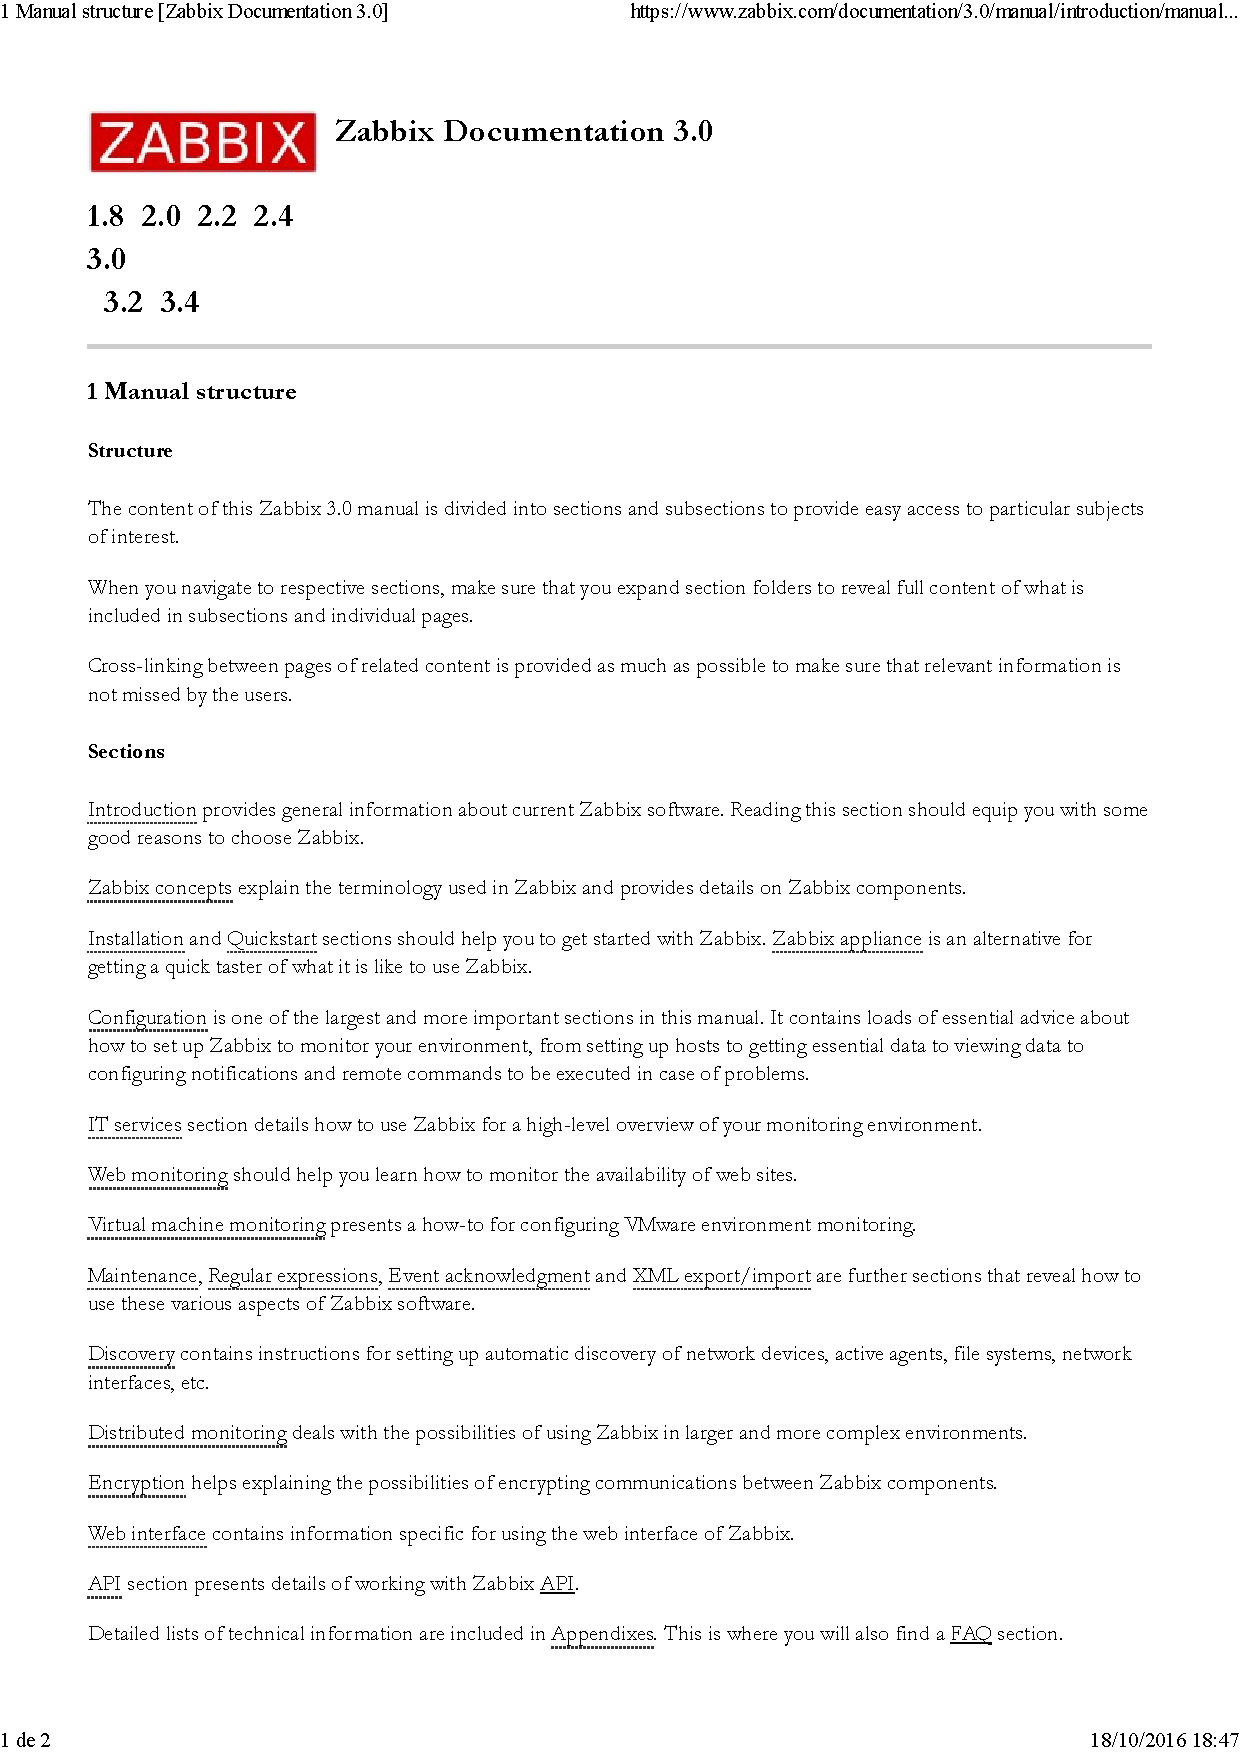
\includegraphics[width=15cm, height=7cm]{1}
\\
Para simular los carros simplemente coloreamos dándole un significado diferente. el color rojo es para los carros que tiene una velocidad 0 que quiere decir que est\'an en alto
\\ \\
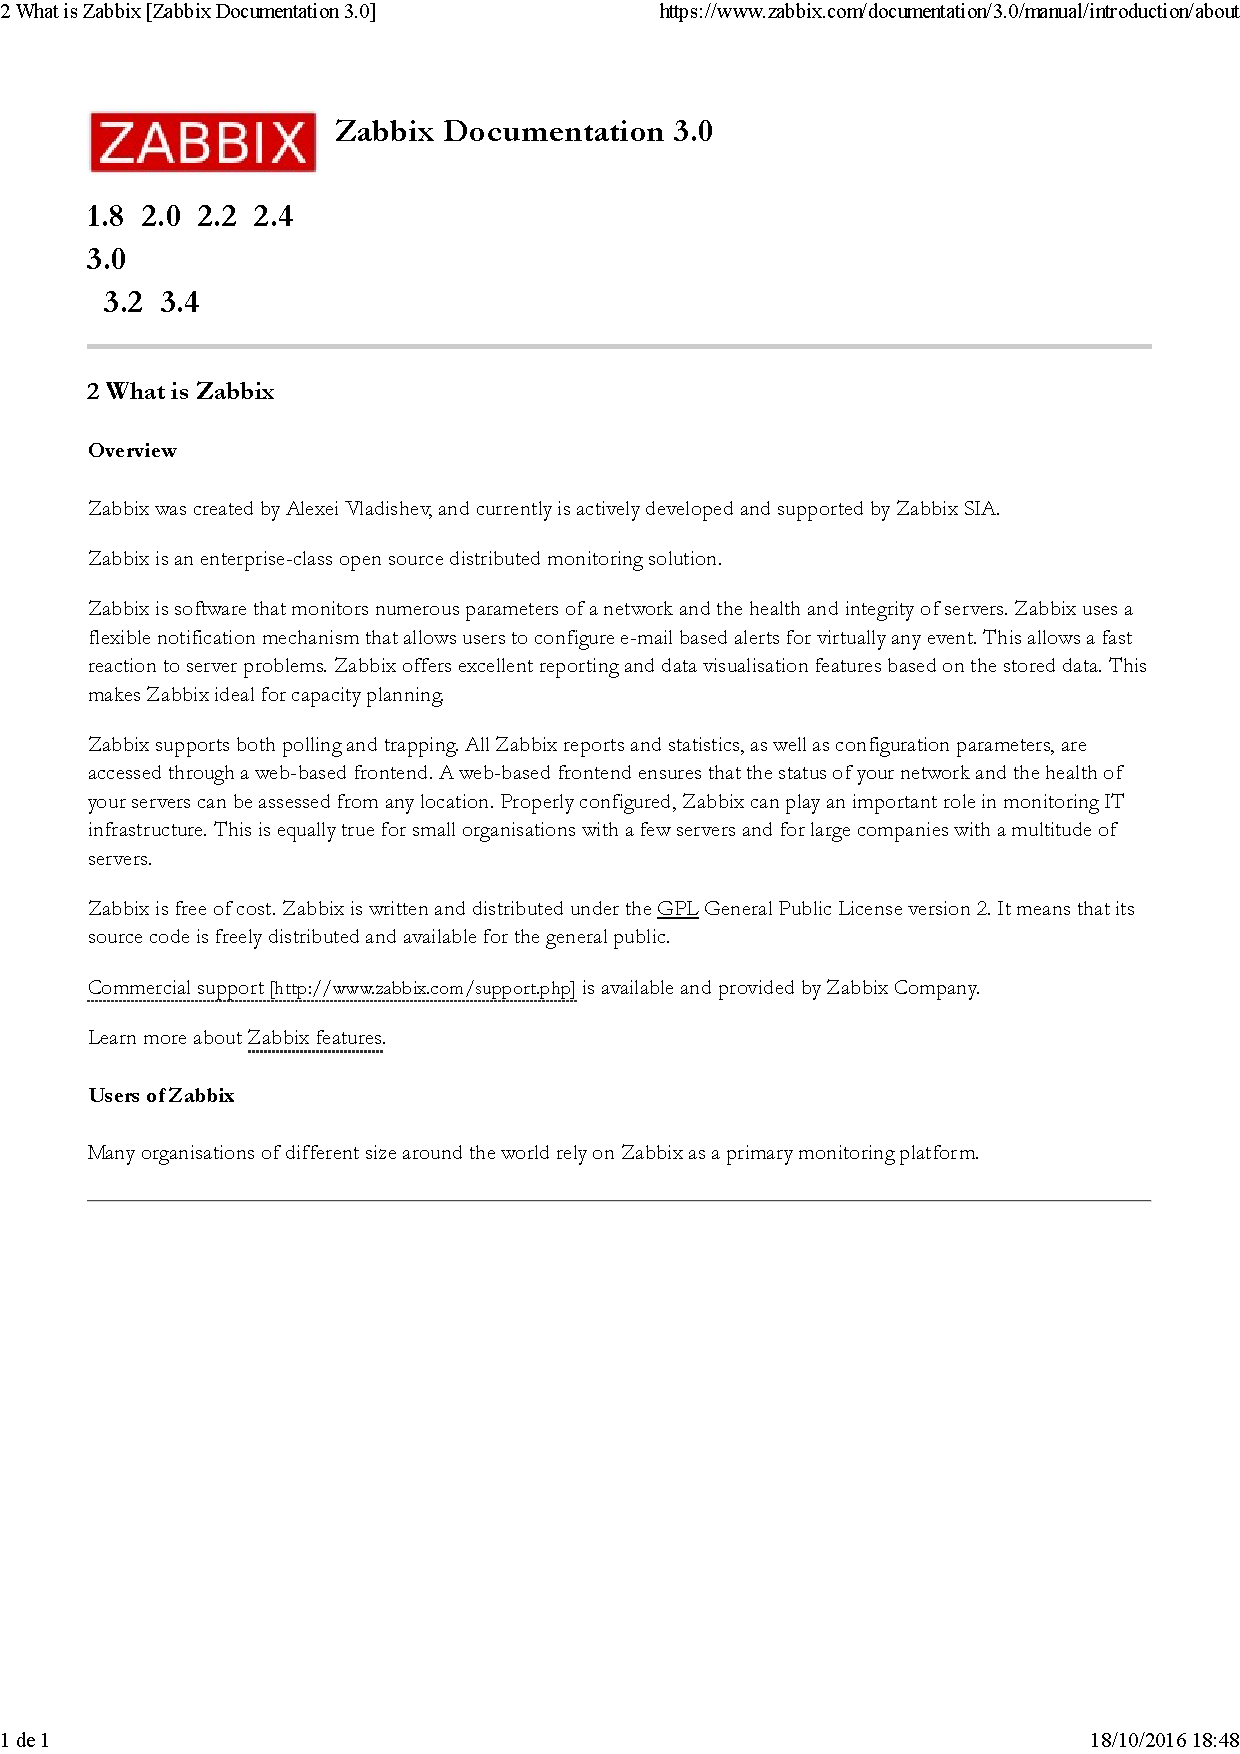
\includegraphics[width=15cm, height=7cm]{2}
\\
Los carros en movimiento son los carros en color verde
\\ \\
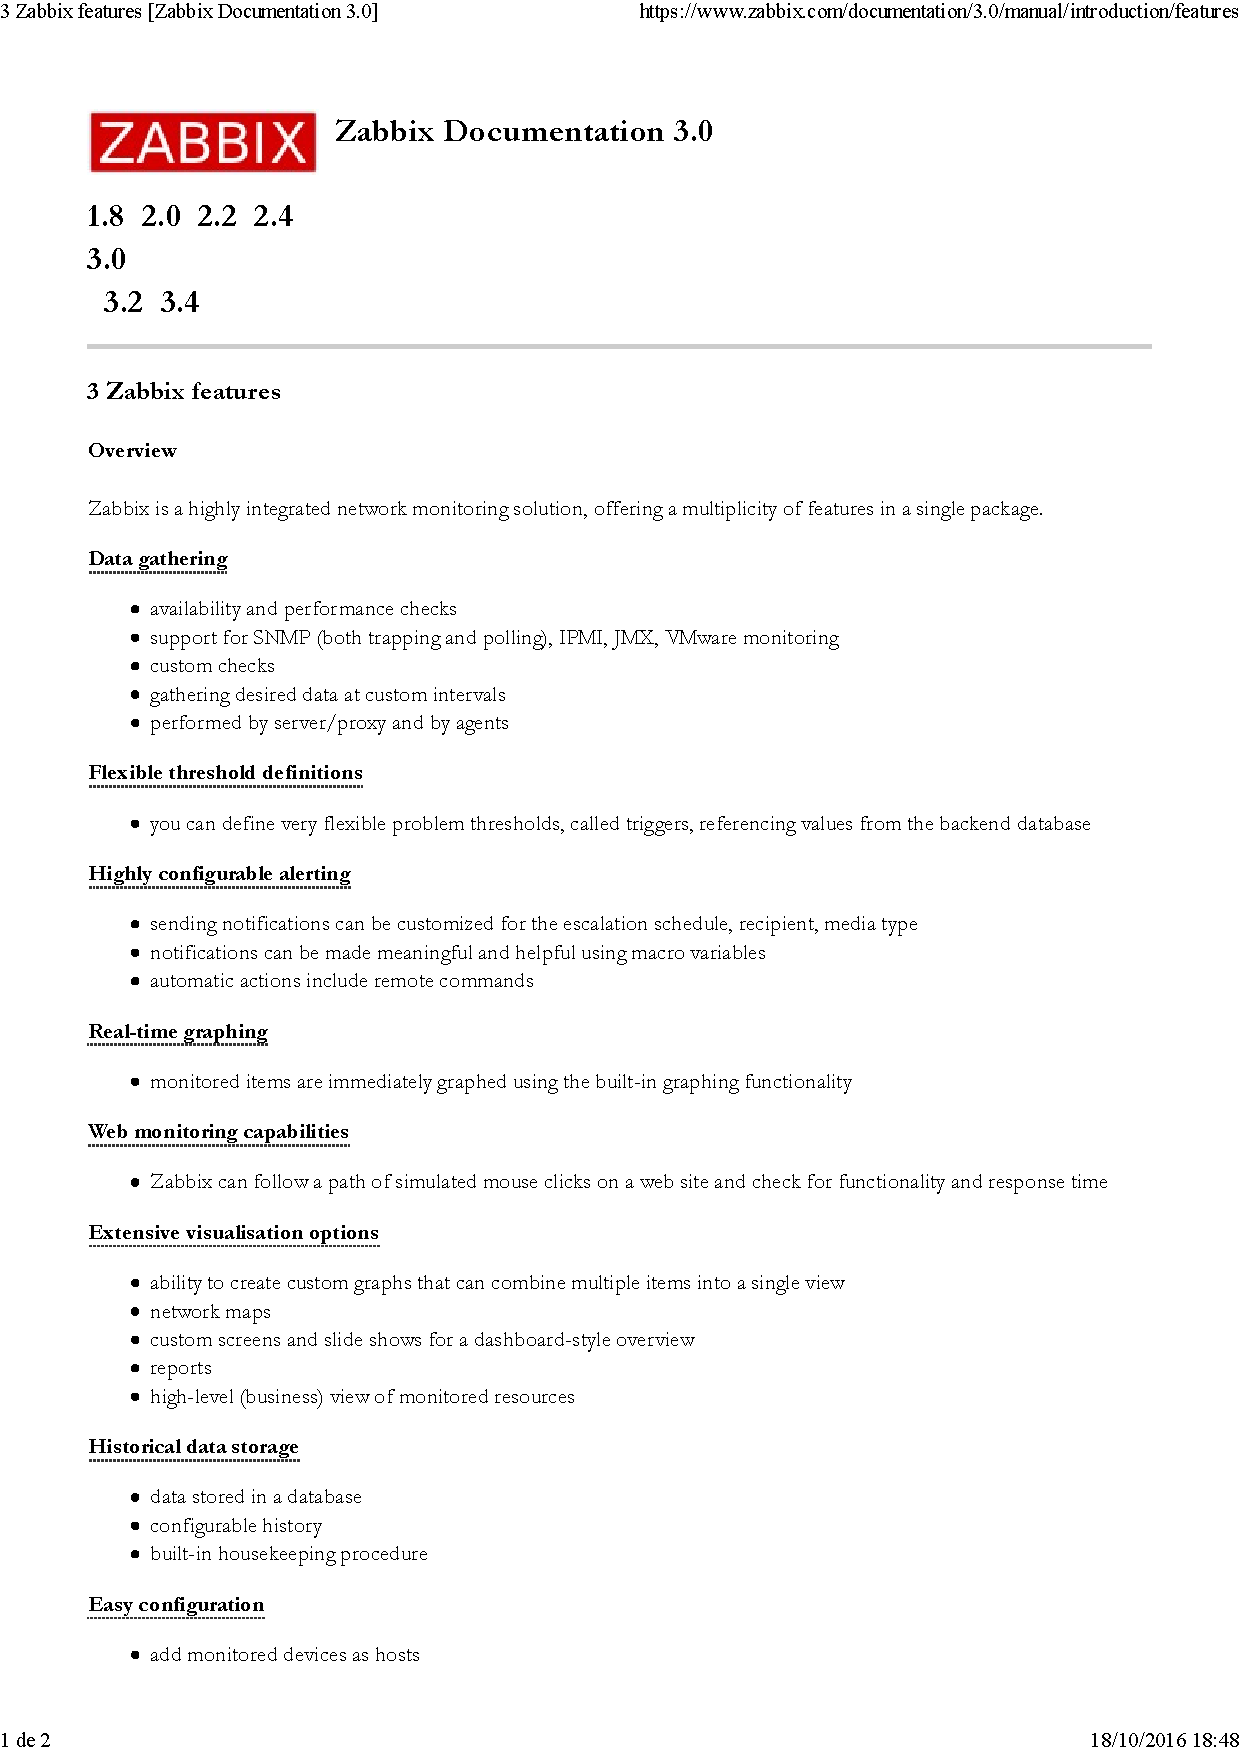
\includegraphics[width=15cm, height=7cm]{3}
\\
\section{Pruebas una sola linea}
Para comprobar que el modelo funciona se le sometio a pruebas probandolo con diferentes dencidades, velocidades maximas y probabilidades 
de tal forma que se pudiera ver como se comporta el trafico.\\ \\
\subsection{Prueba 1}
La primera prueba es con una dencidad de 2\%, una velocidad Maxima de 135km/h y probabilidad de paro de 0\%.
\\ \\
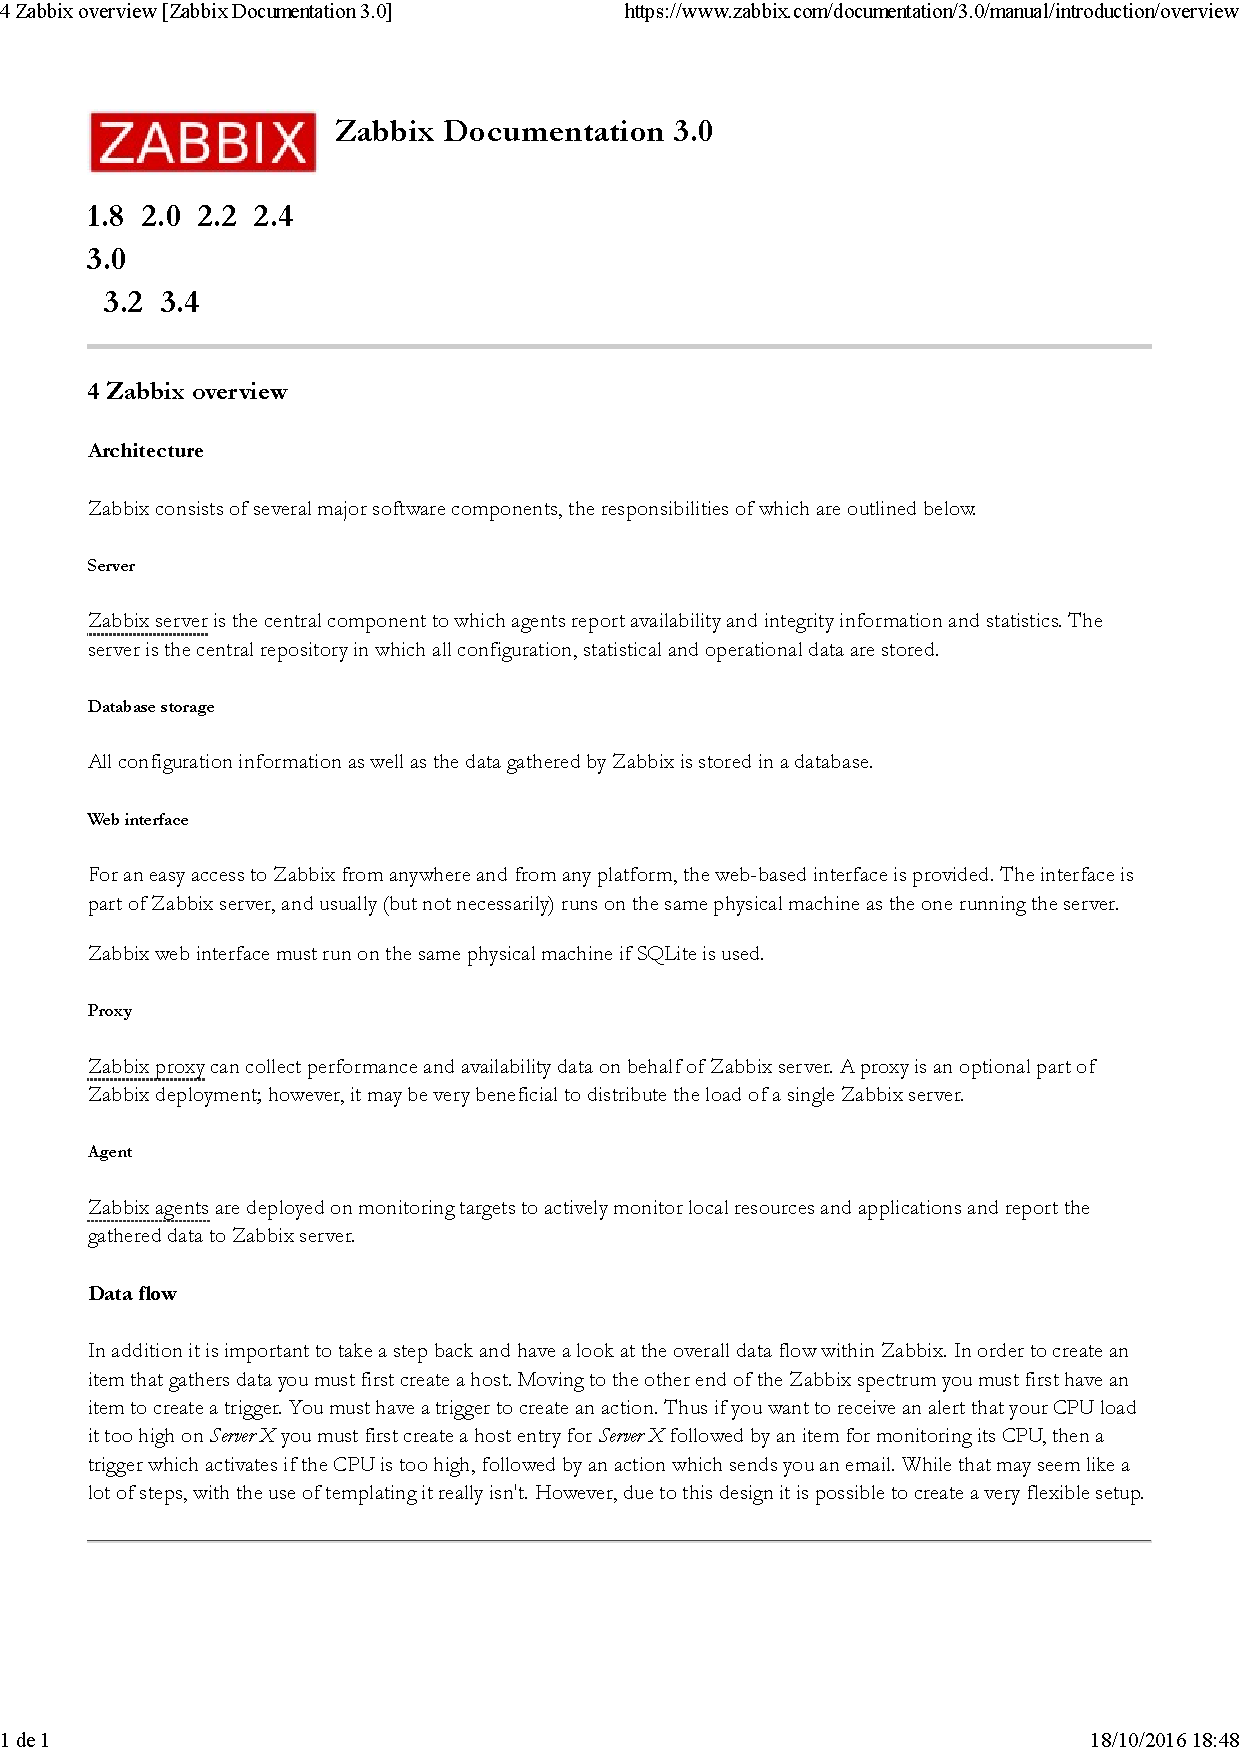
\includegraphics[width=15cm, height=7cm]{4}
\\ \\
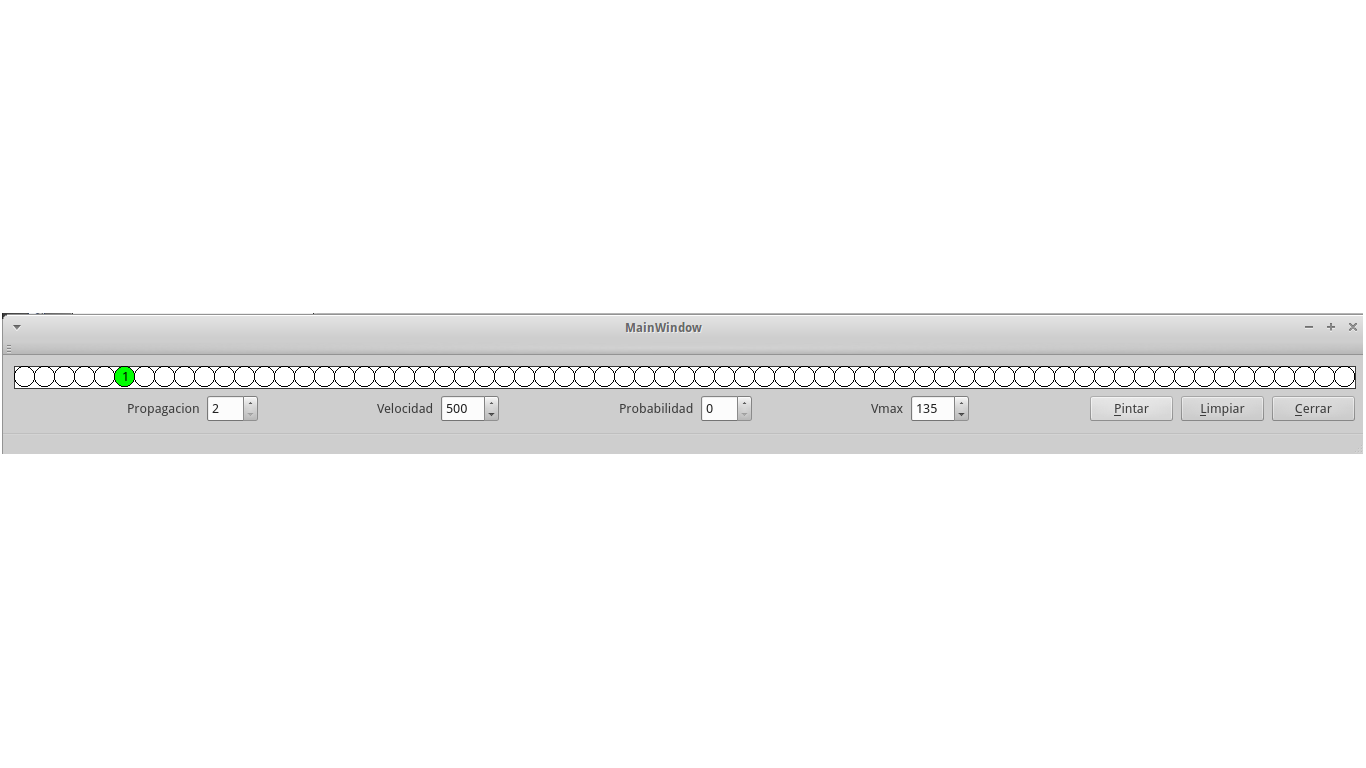
\includegraphics[width=15cm, height=7cm]{5}
\\ \\
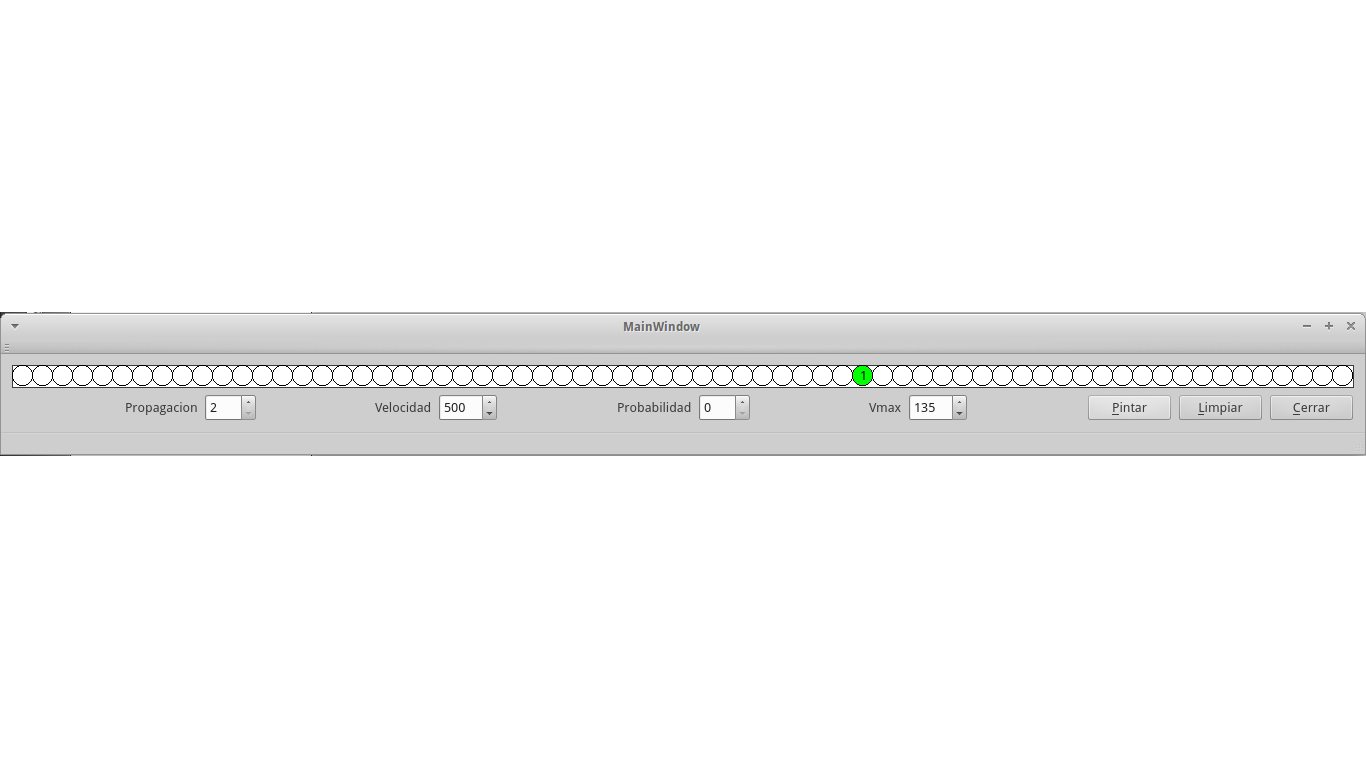
\includegraphics[width=15cm, height=7cm]{6}
\\ \\
Podemos ver que como solamente tenemos un auto en la carretera es imposible que se cree un embotellamiento, y aun que se le agregara 
probabilidad tal vez se pararia el carro pero despues seguiria su marcha.
\subsection{Prueba 2.1}
Densidad de 5\% Vmax 135Km/h probabilidad de paro 0%
\\ \\
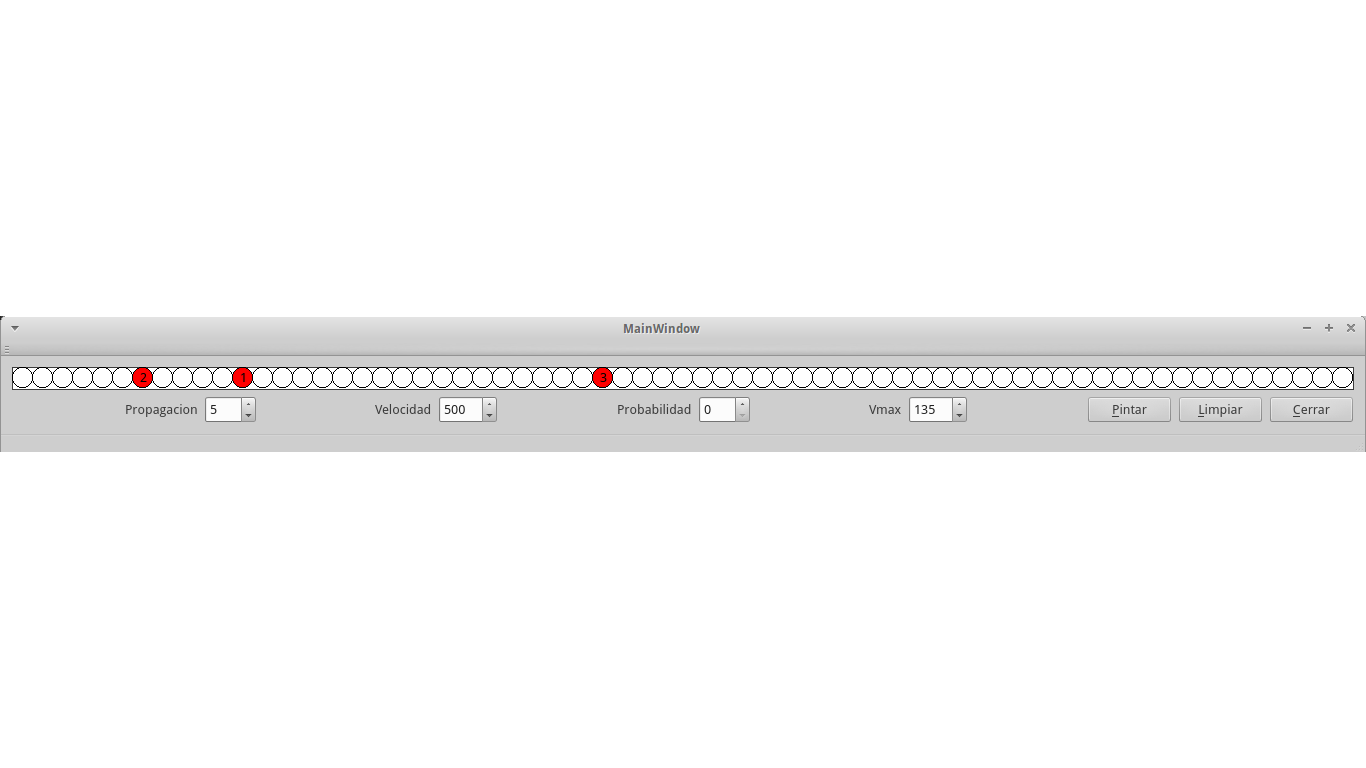
\includegraphics[width=15cm, height=7cm]{7}
\\ \\
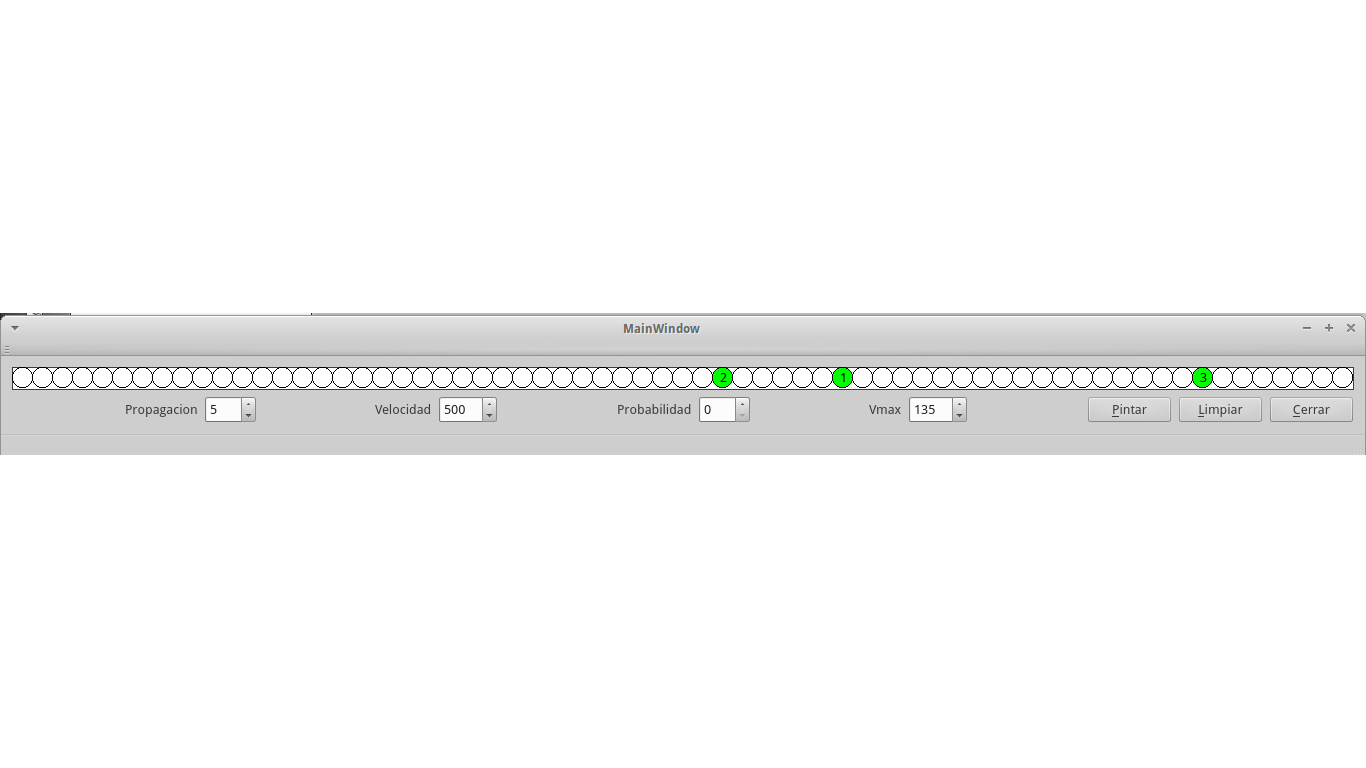
\includegraphics[width=15cm, height=7cm]{8}
\\ \\
Tenemos ahora 3 autos pero como se encuentran a una distancia considerable por lo tanto pueden seguir sin problema. Probemos con probabilidad.
\subsection{Prueba 2.2}
Densidad de 5\% Vmax 135Km/h probabilidad de paro 60\%
\\ \\
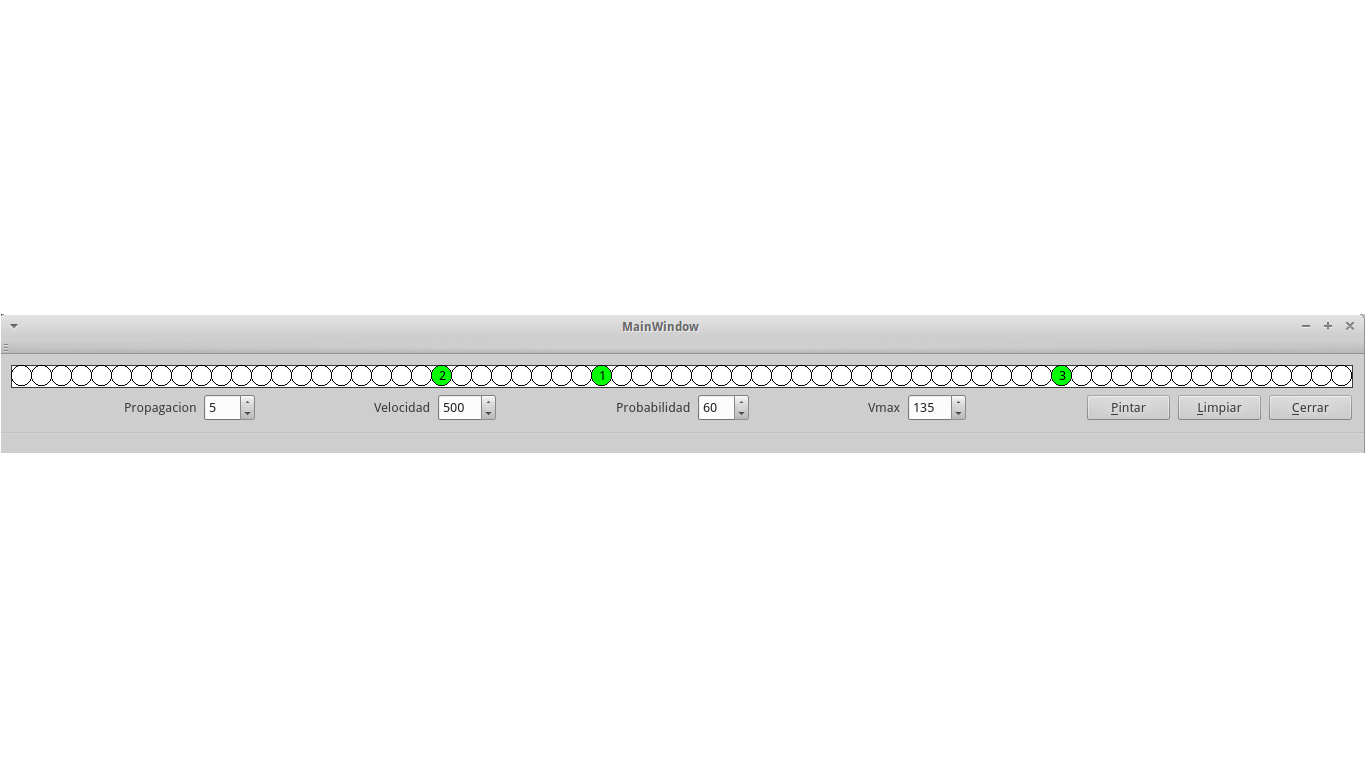
\includegraphics[width=15cm, height=7cm]{9}
\\ \\
Aun que se uso la probabilidad por la distancia a la que se encuentran los elementos esto no afecta.
\subsection{Prueba 3.1}
Densidad 10\% Vmax 135Km/h probabilidad de paro 0\%
\\ \\
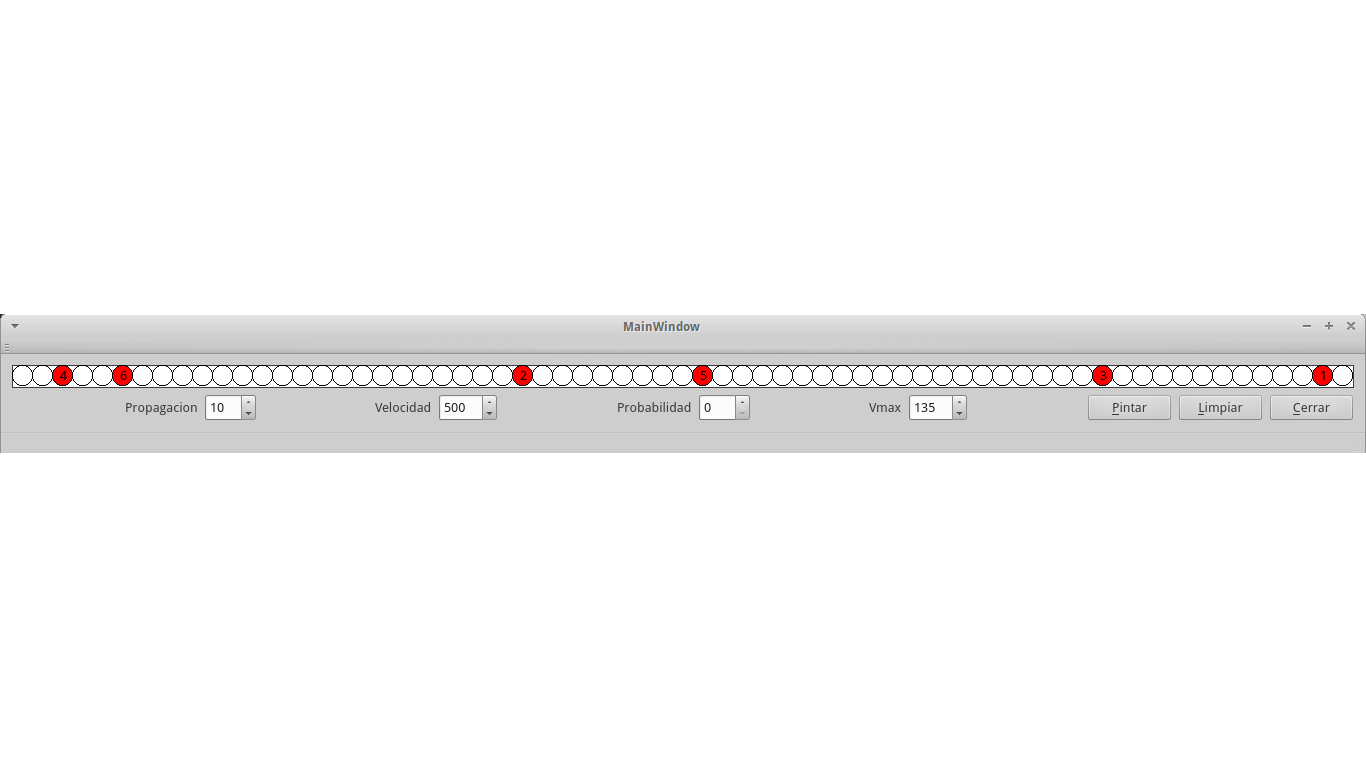
\includegraphics[width=15cm, height=7cm]{10}
\\ \\
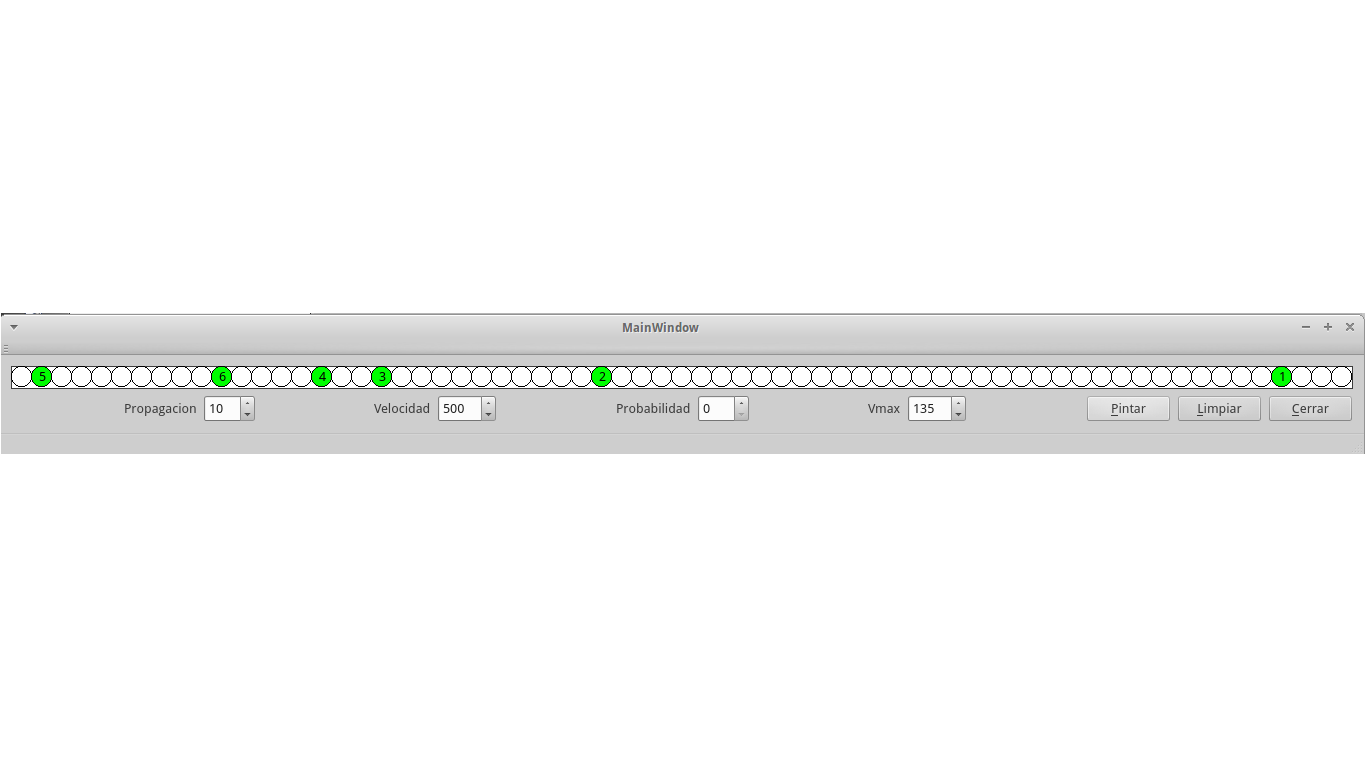
\includegraphics[width=15cm, height=7cm]{11}
\\ \\
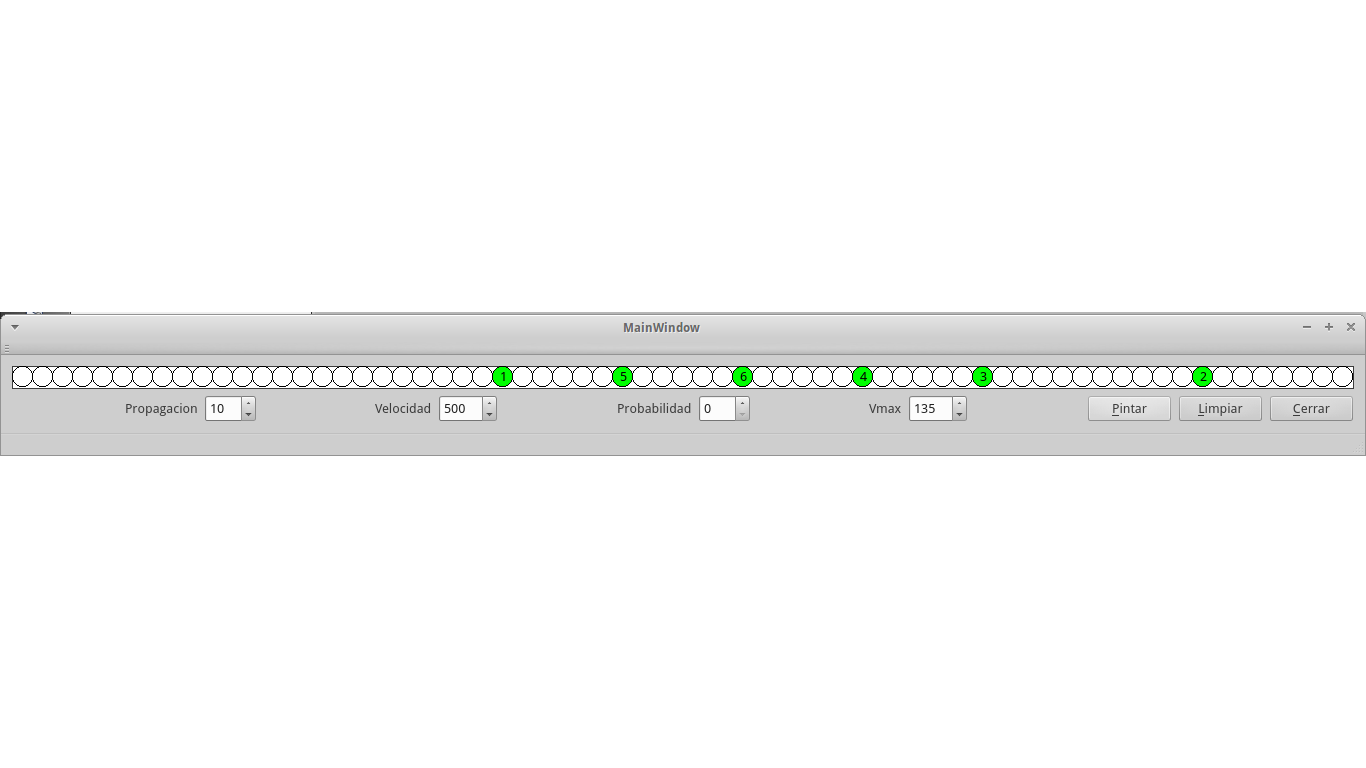
\includegraphics[width=15cm, height=7cm]{12}
\\ \\
Vemos 6 autos que se mantienen a una distancia constante entre ellos pero si mandamos la misma configuracion con probabilidad de paro el comportamiento cambia.
\\ \\
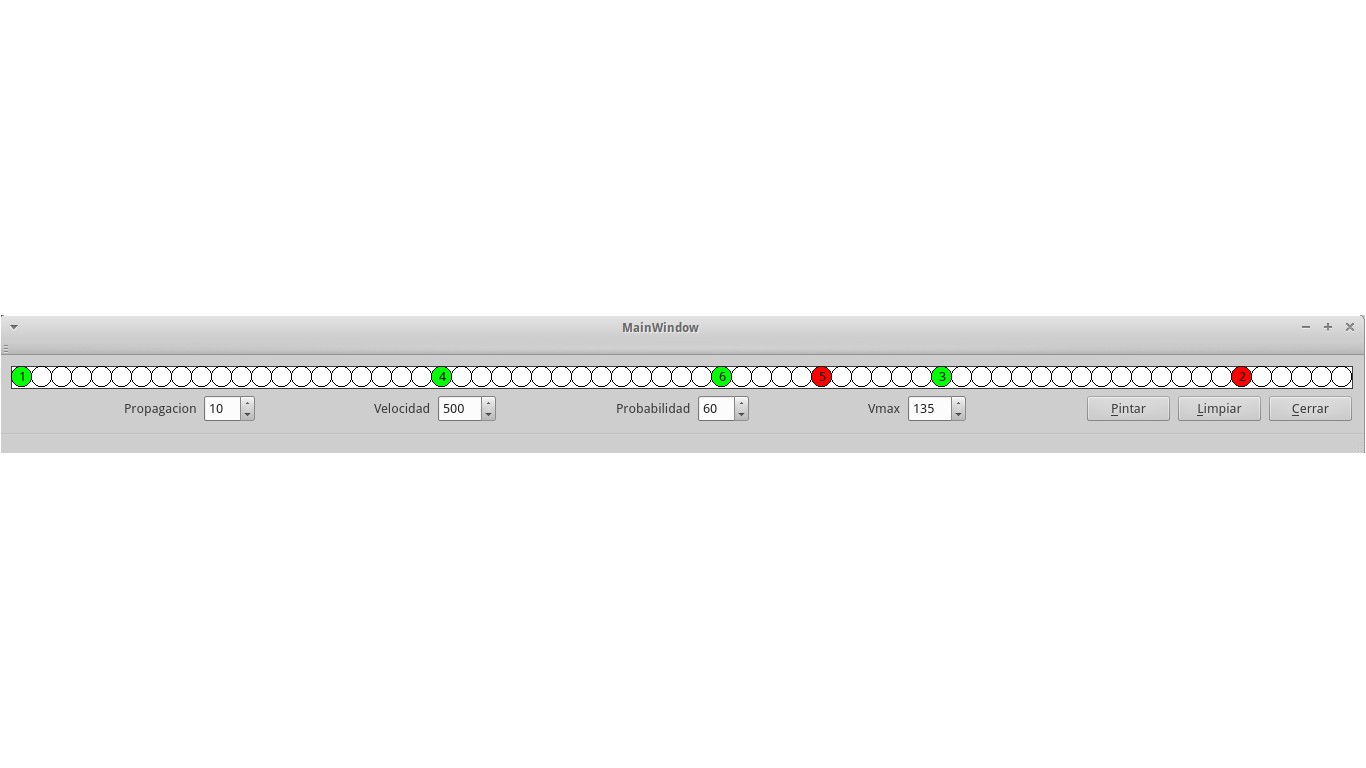
\includegraphics[width=15cm, height=7cm]{13}
\\ \\
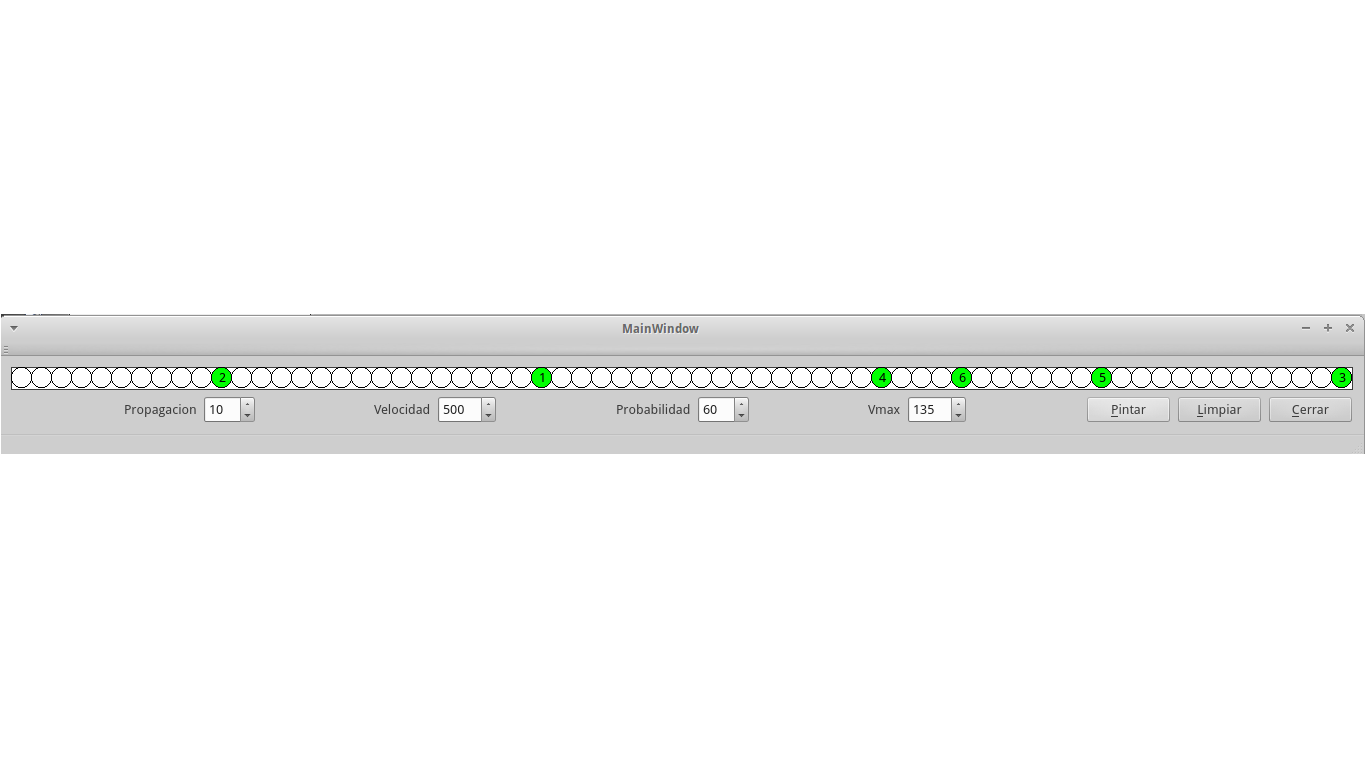
\includegraphics[width=15cm, height=7cm]{14}
\\ \\
En este caso se crea un pequeño atoron pero despues de unos ciclos el sistema fluye como cuando no tiene probabilidad.
\subsection{Prueba 4.1}
Densidad 20\% Vmax 135km/h probabilidad 0\%
\\ \\
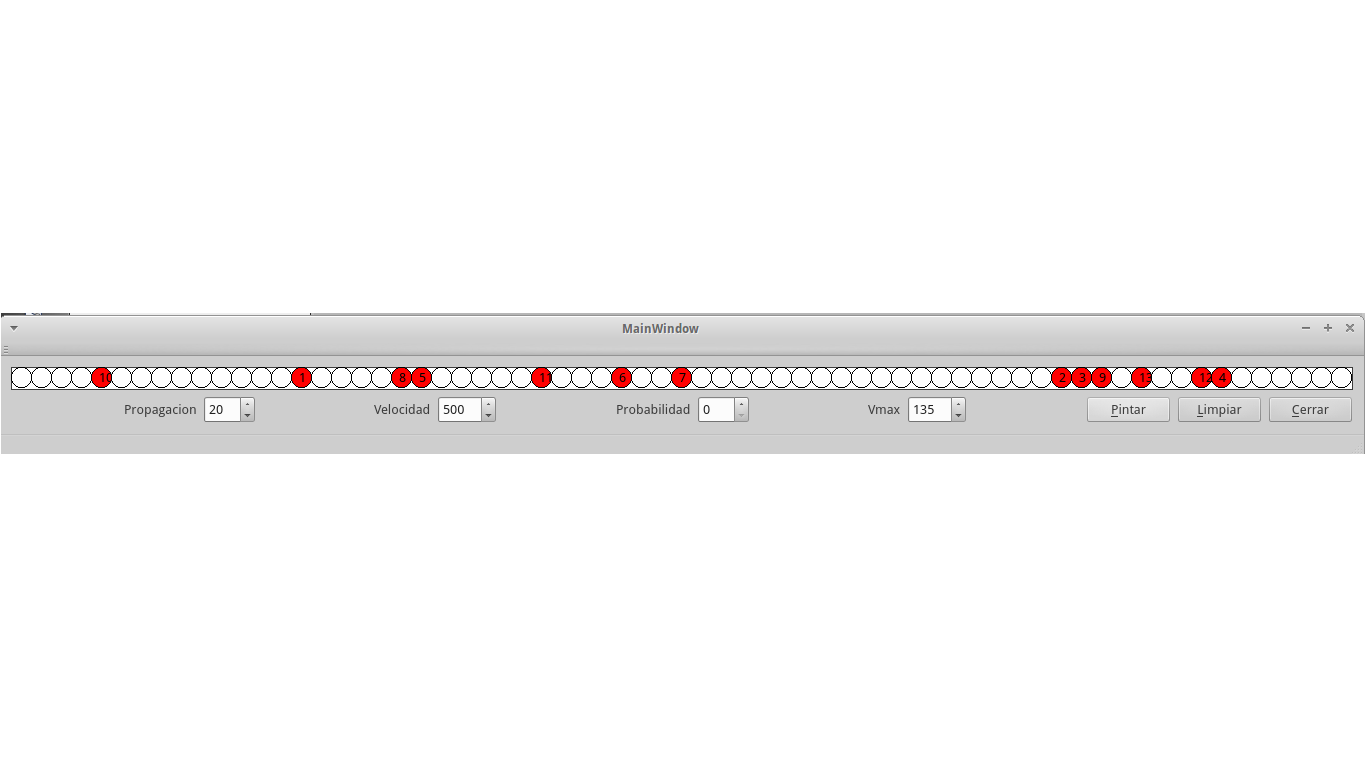
\includegraphics[width=15cm, height=7cm]{15}
\\ \\
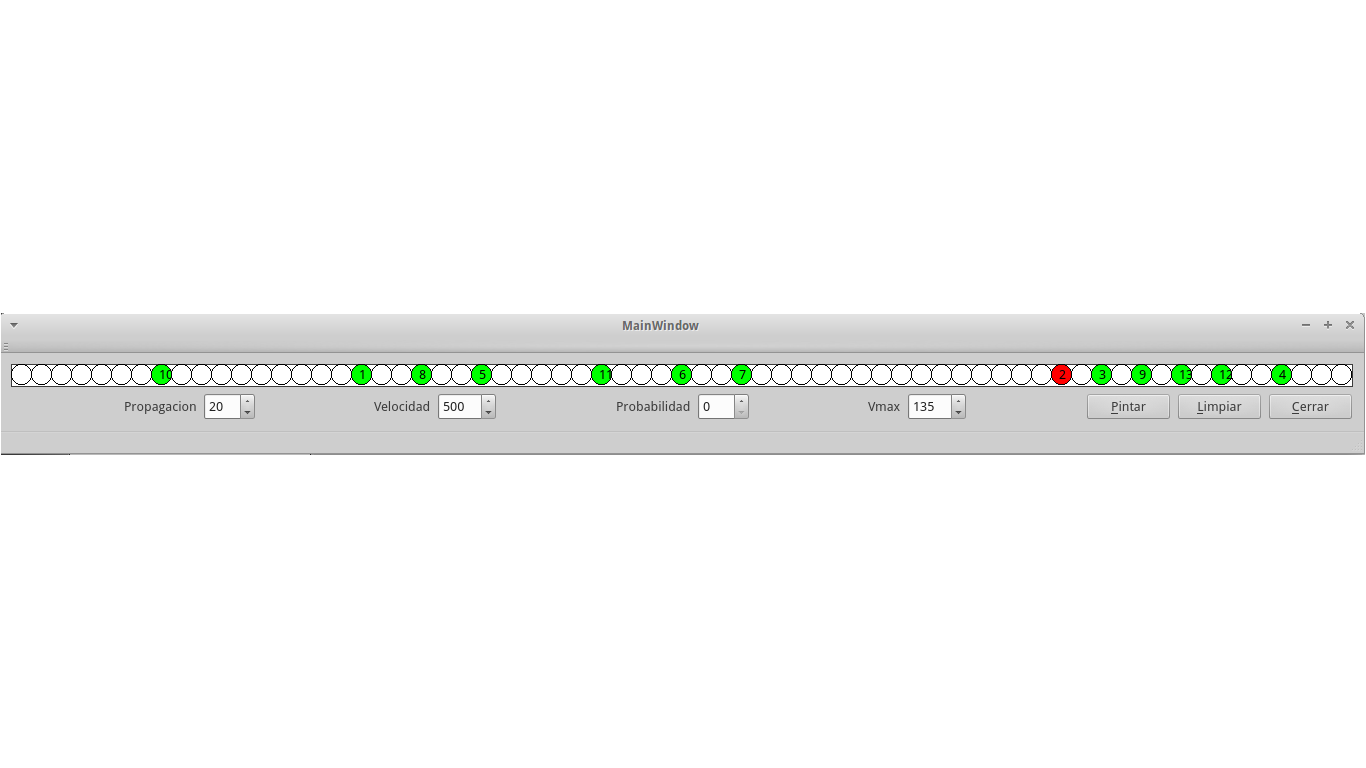
\includegraphics[width=15cm, height=7cm]{16}
\\ \\
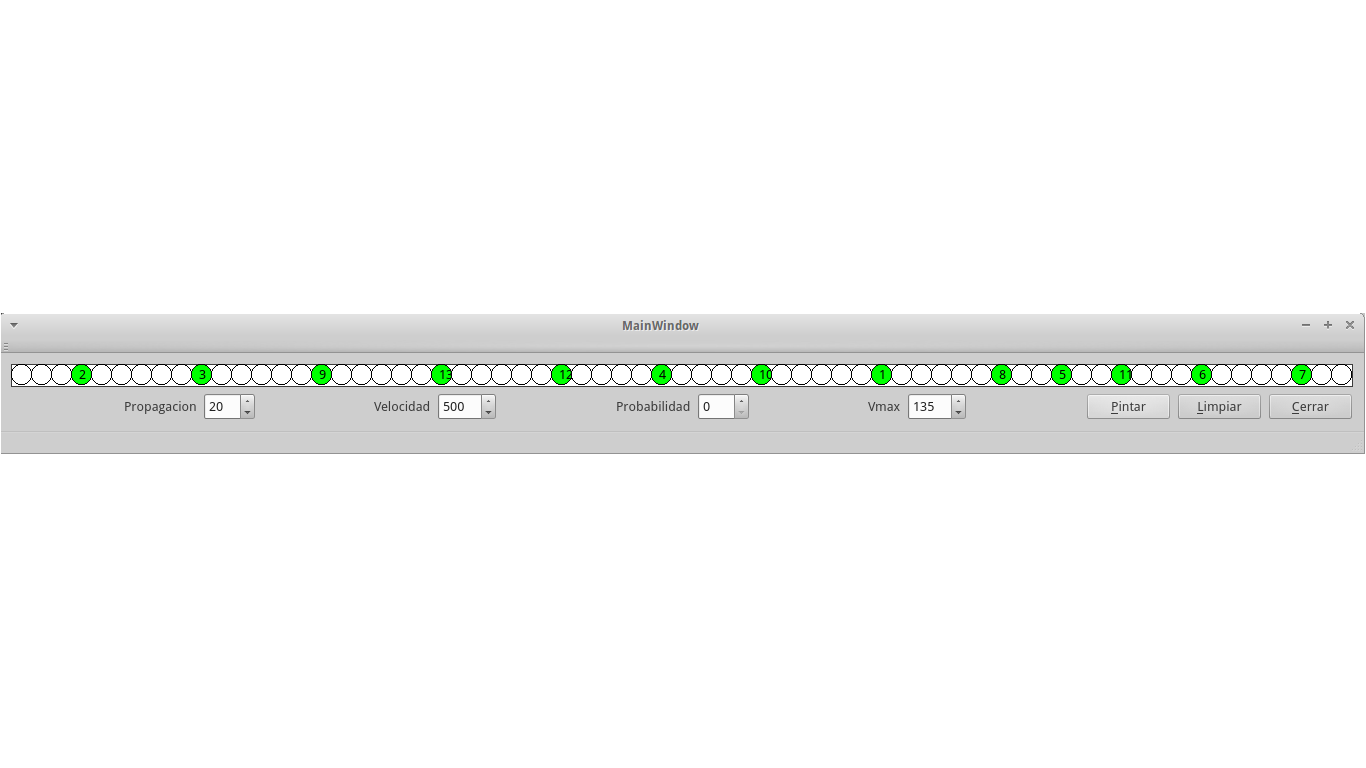
\includegraphics[width=15cm, height=7cm]{17}
\\
En este caso existen atorones al principio pero el sistema se estabiliza y continua normalmente.\\
al incuir una prbabilidad del 60\% de paro veremos el siguiente comportamiento.
\\ \\
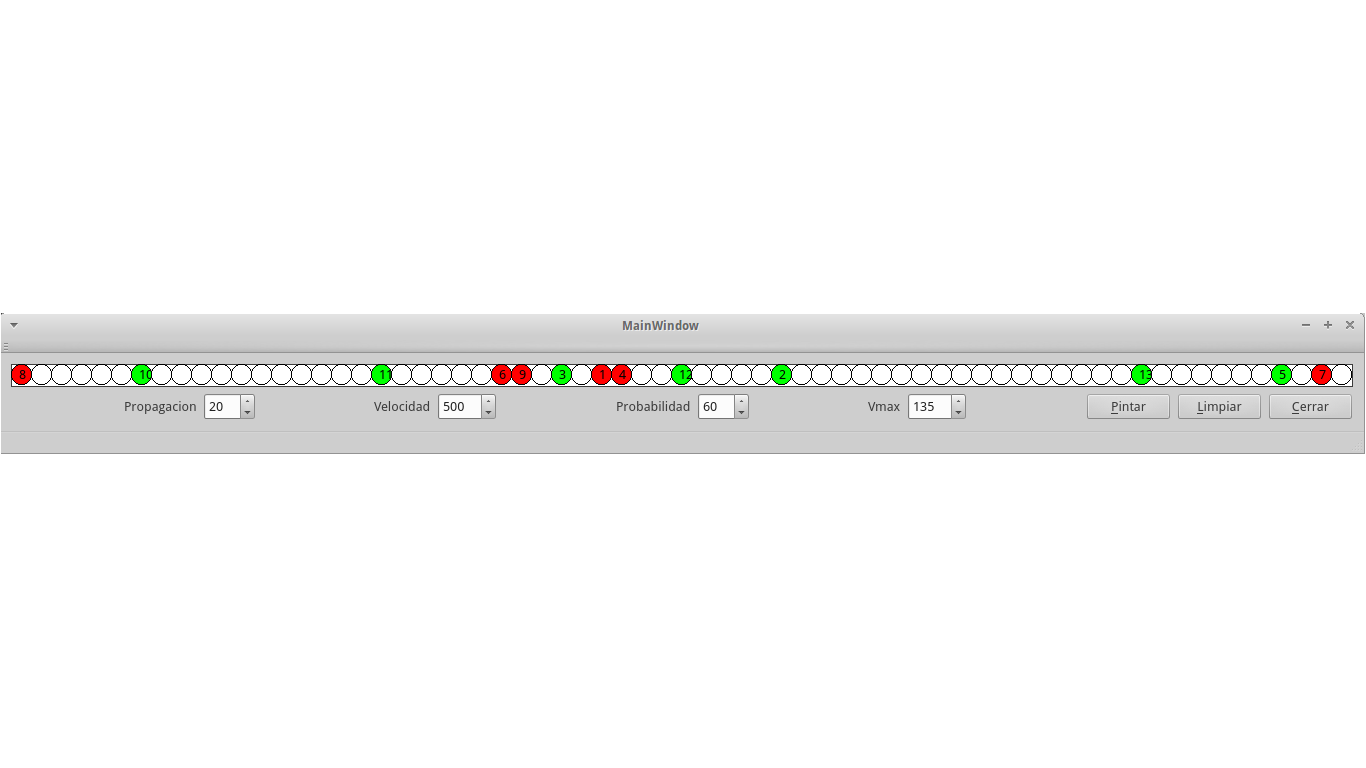
\includegraphics[width=15cm, height=7cm]{22}
\\
Podemos ver que se crean atorones desde el principio del sistema y no solo 1 si no que 3 atorones al mismo tiempo, este comportamiento continua en el sistema y no desaparece.
\subsection{Prueba 5}
Densidad 30\% Vmax 135km/h probabilidad 0\%
\\
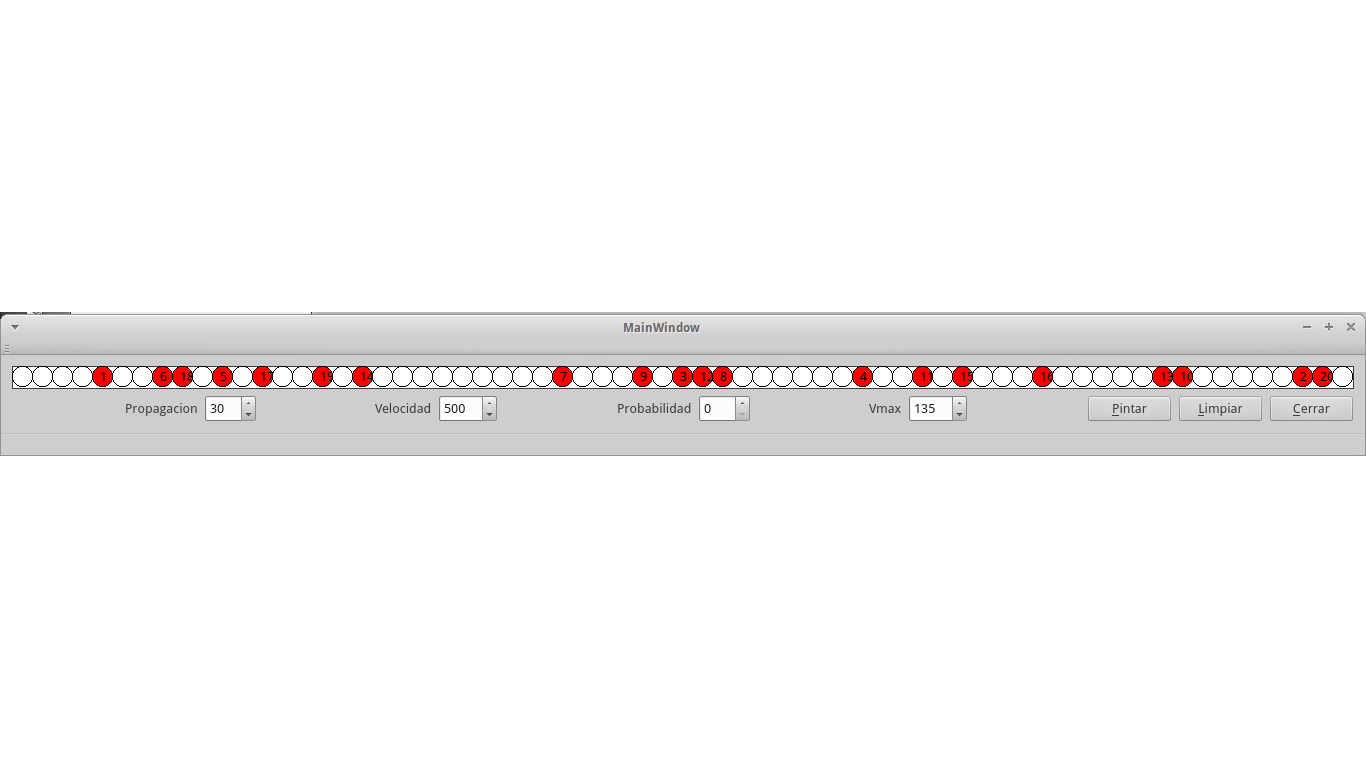
\includegraphics[width=15cm, height=7cm]{18}
\\
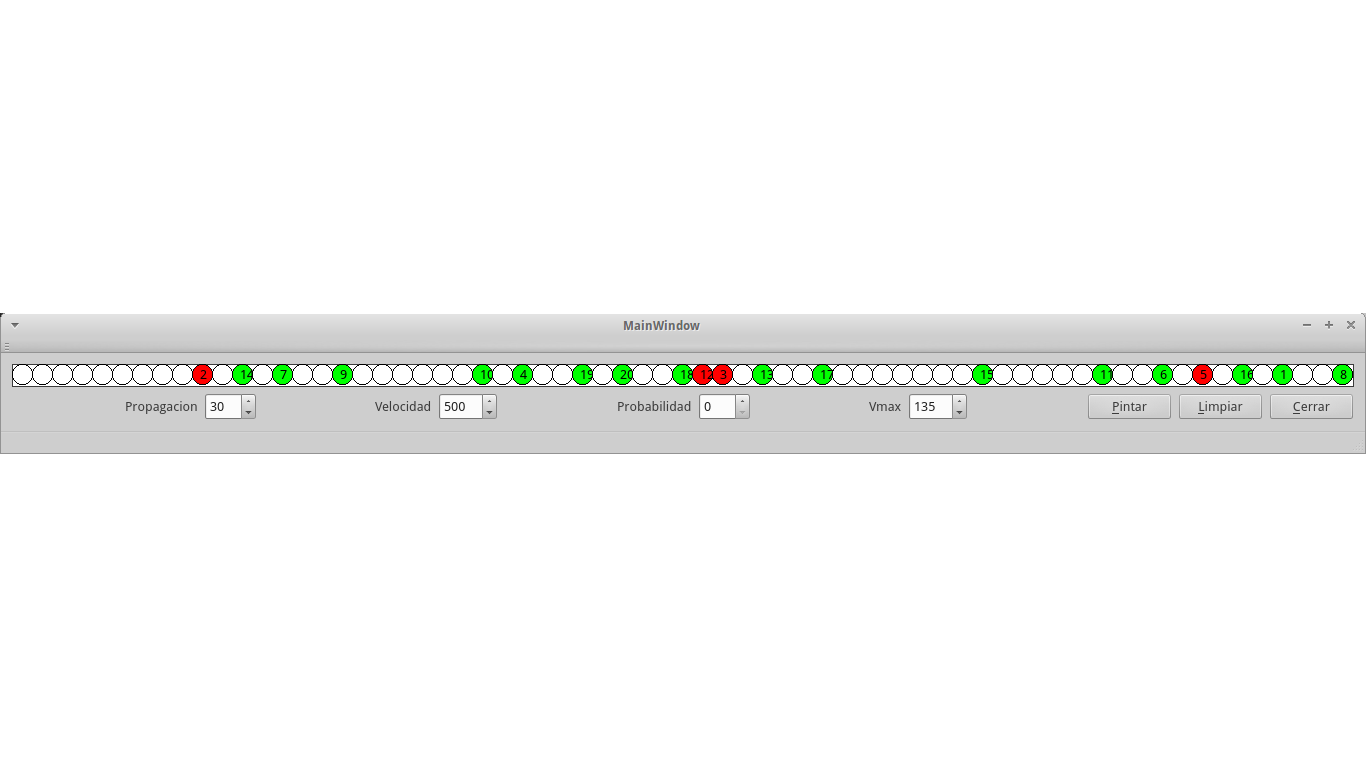
\includegraphics[width=15cm, height=7cm]{19}
\\
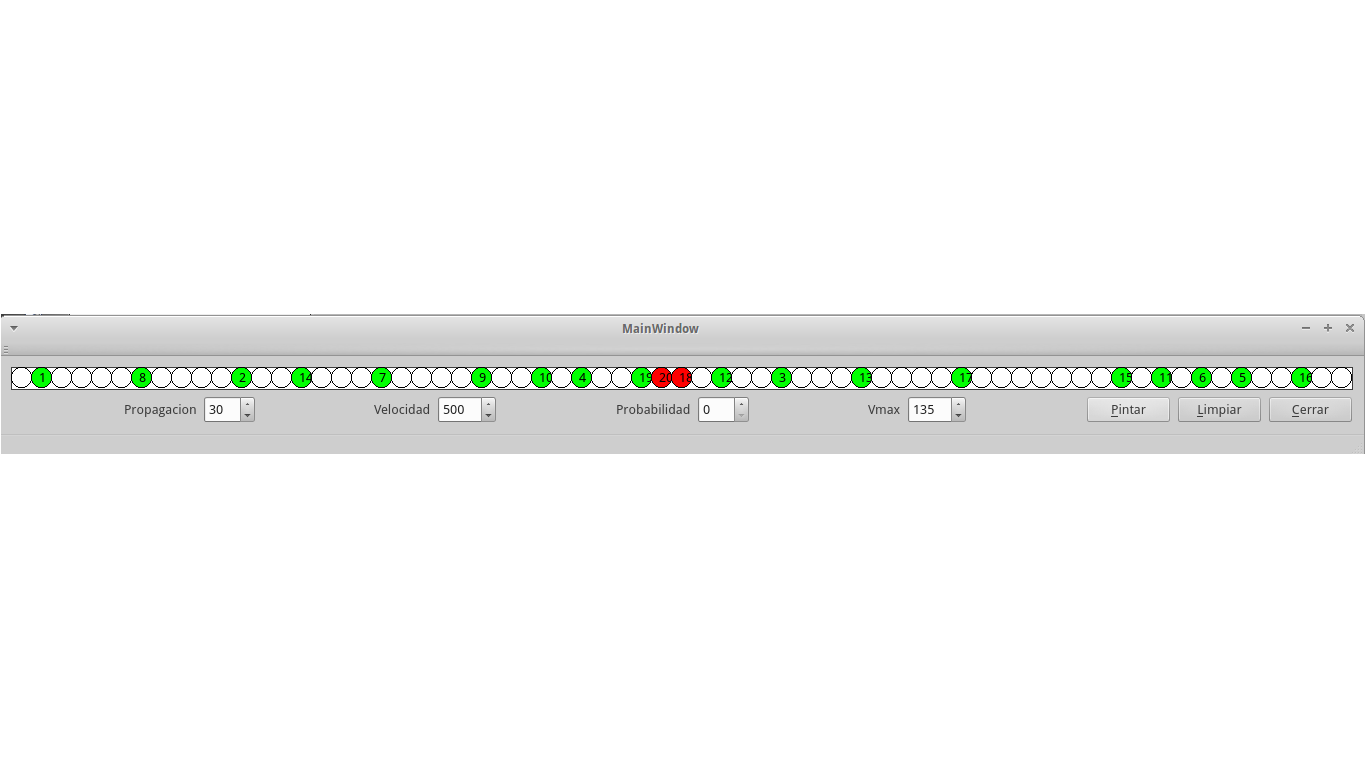
\includegraphics[width=15cm, height=7cm]{20}
\\
Se crea una toron desde el principio del sistema y aun que todabia no le agregamos probabilidad, este atoron continua en el sistema y no desaparece. Este fenomeno sucede en la realidad cuando una persona cruza la calle cuando no debe y genera un trafico minimo que se recorre en la calle.
\subsection{Prueba 6}
Densidad 40\% Vmax 135km/h probabilidad 0\%
\\
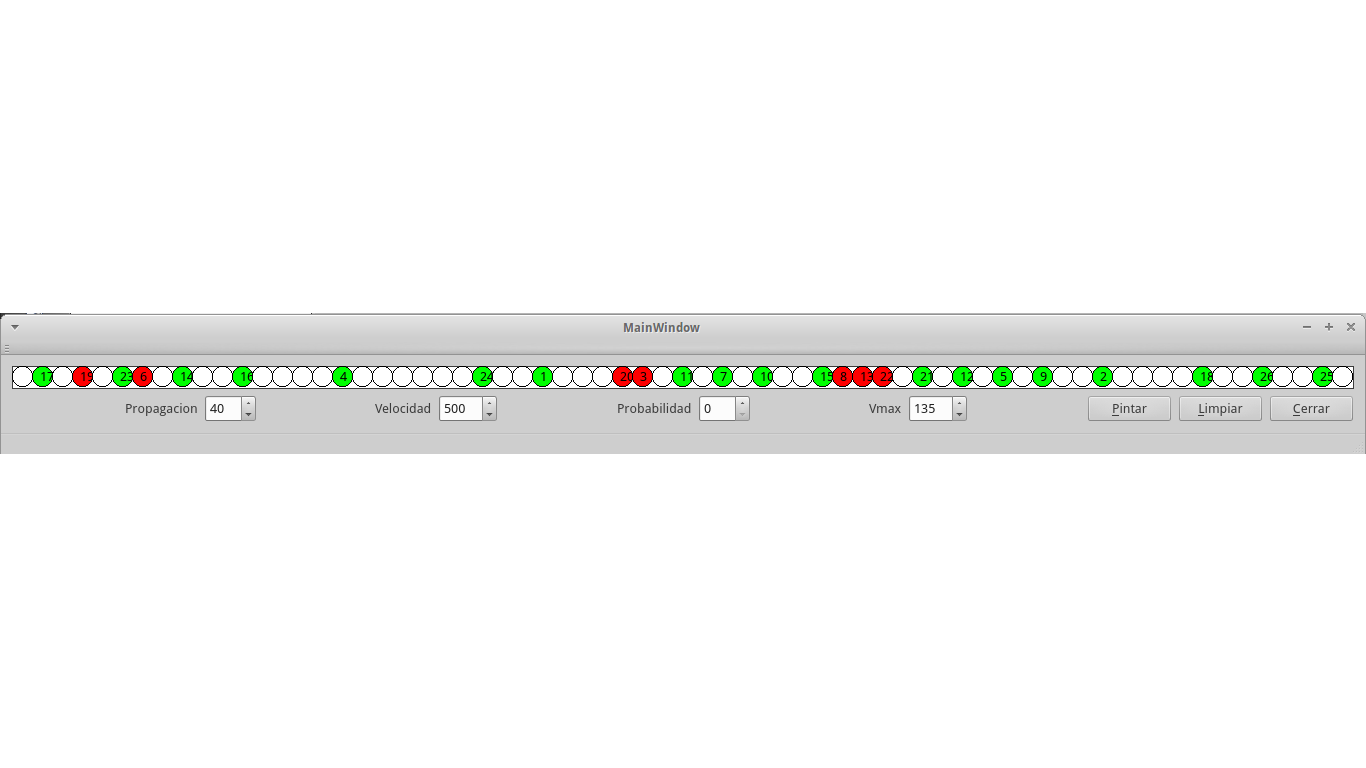
\includegraphics[width=15cm, height=7cm]{23}
\\
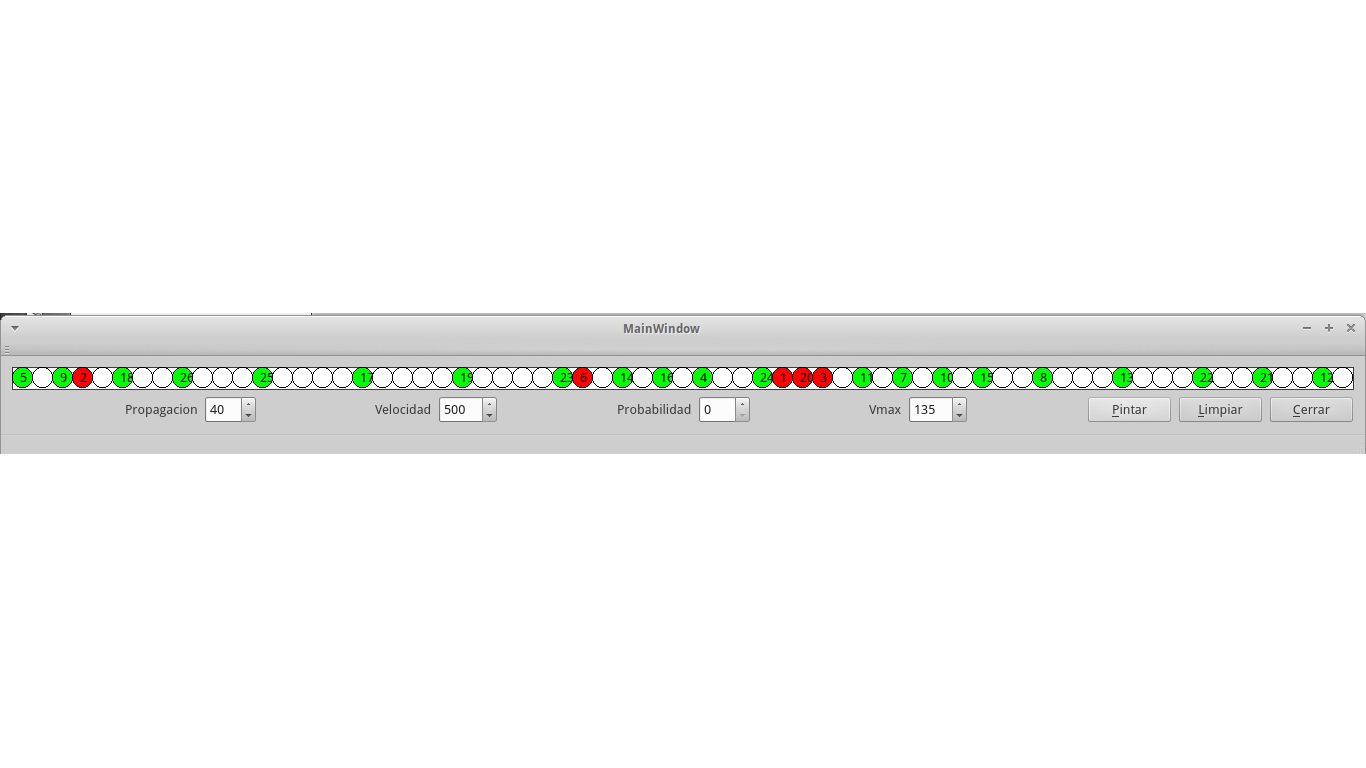
\includegraphics[width=15cm, height=7cm]{24}
\\
En este caso se crean atorones desde el principio y estos no desaparecen, este tipo de fenomenos son similares a cuando tenemos cruseros con otros carros pero en este caso al no existir esta posibilidad queda descartada siendo un caso extendido de la prueba anterior.\\
Si agregamos probailidad podremos ver lo siguiente.
\\
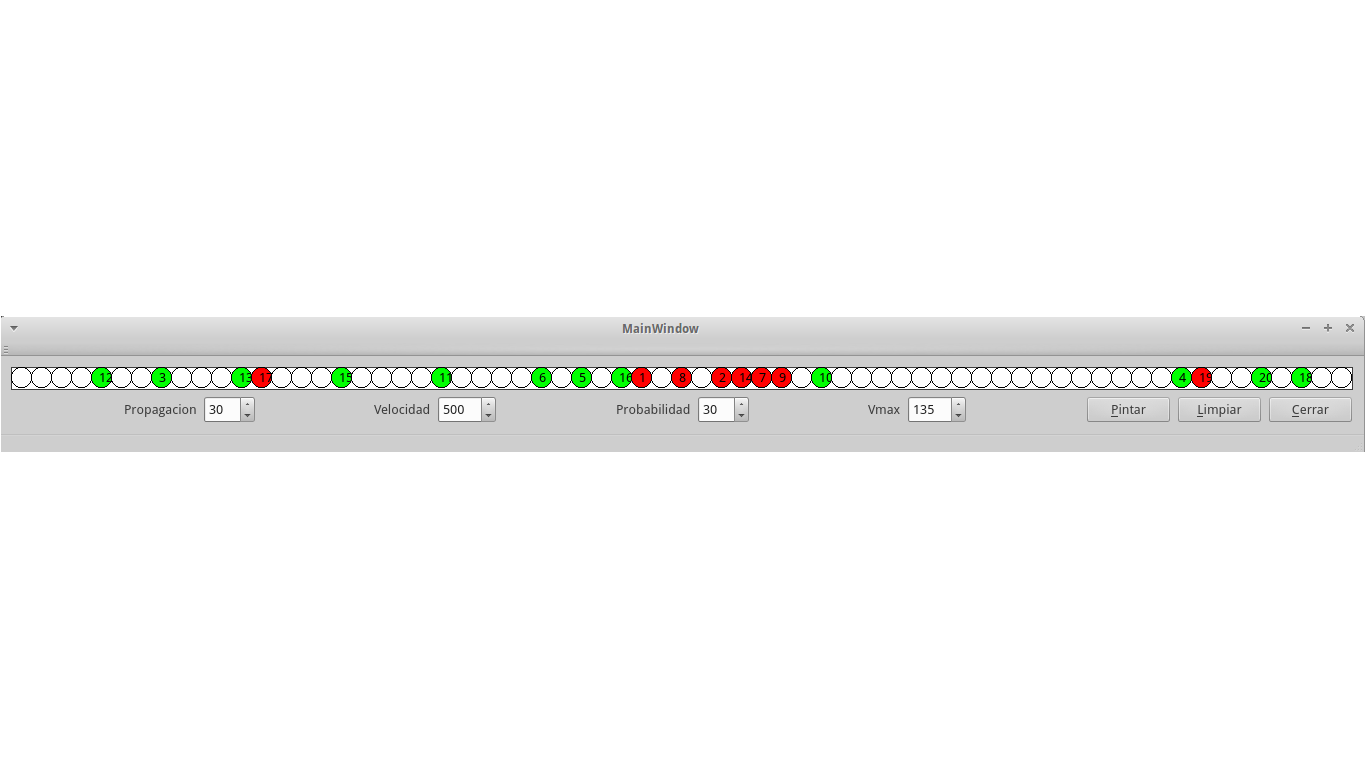
\includegraphics[width=15cm, height=7cm]{21}
\\
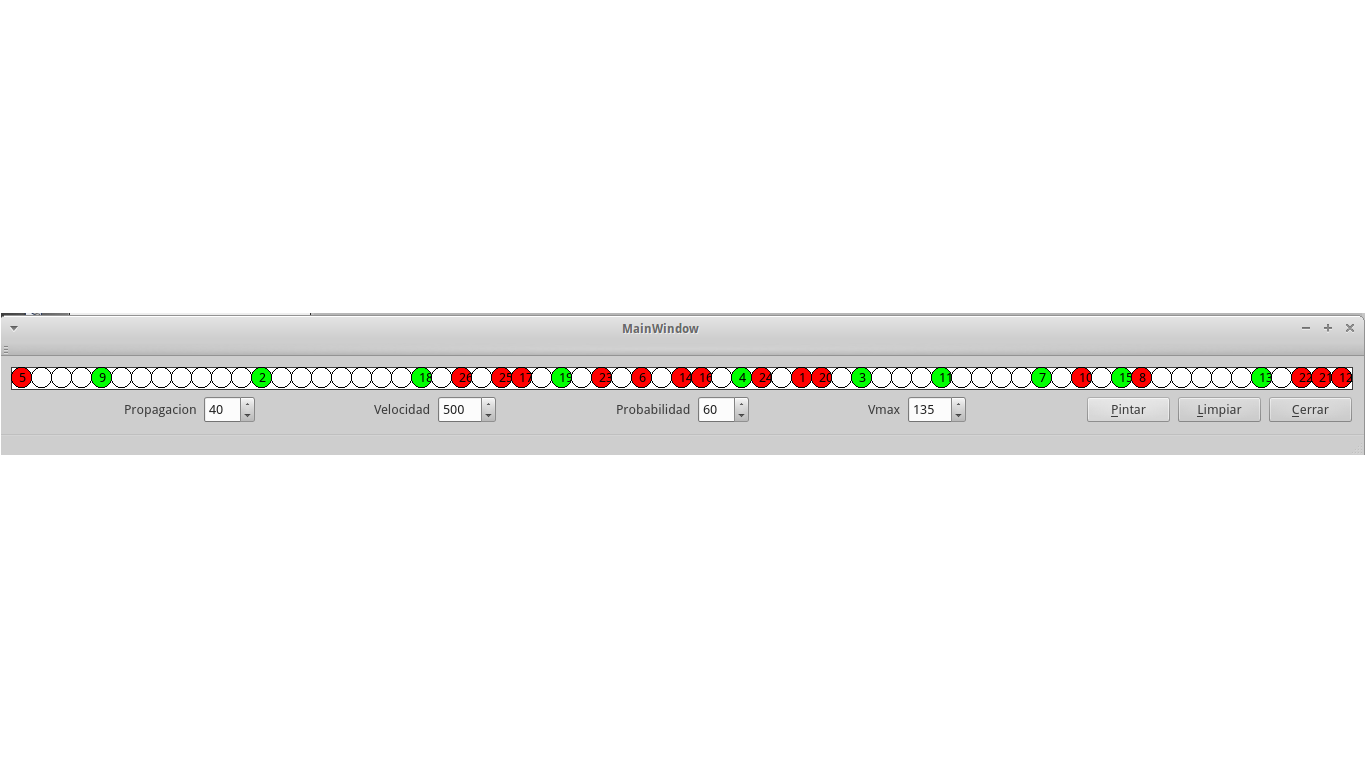
\includegraphics[width=15cm, height=7cm]{25}
\\
se le agrega una probailidad de 30\% y del 60\% correspondientemente y podemos ver que casi se para el trafico, podemos ver si seguimos varios ciclos de este caso que los estancamientos se generan en el mismo lugar pudiera ser un comportamiento similar al que cuando hay cemaforos peatonales.
\subsection{Prueba 7}
Densidad 50\% Vmax 135km/h probabilidad 0\%
\\
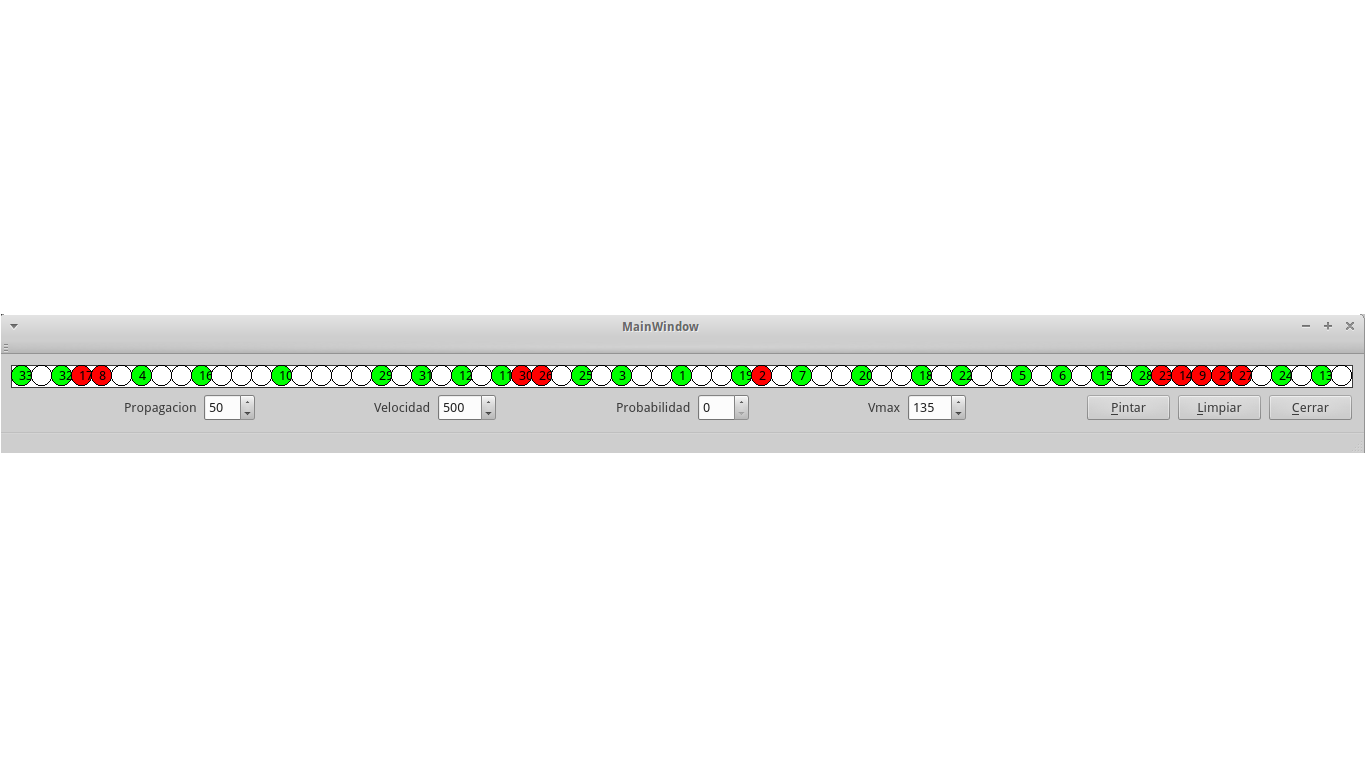
\includegraphics[width=15cm, height=7cm]{26}
\\

Podemos ver a partir de este punto que conforme aumenta la densidad el comportamiento de las pruebas anteriores aunmenta en numero de estancamientos ya que ahora tenemos 4 estancamientos en lugar 3.\\
Cuando agragamos probabilidad surge el siguiente patron.
\\
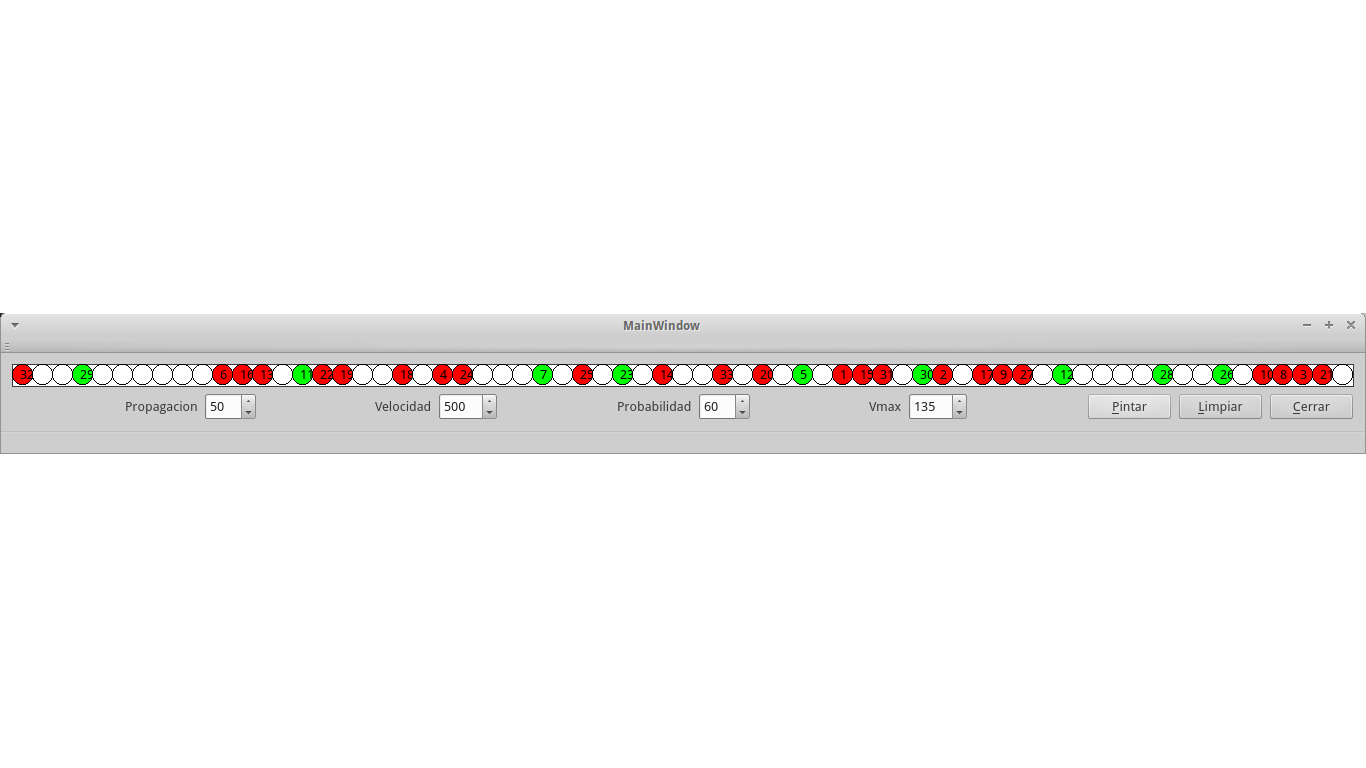
\includegraphics[width=15cm, height=7cm]{27}
\\
Se genera un trafico casi homogeneo en toda la carretera y podemos ver como es que se acumula el trafico unicamente en 2 puntos.
\subsection{Prueba 8}
Densidad 60\% Vmax 135km/h probabilidad 0\%
\\
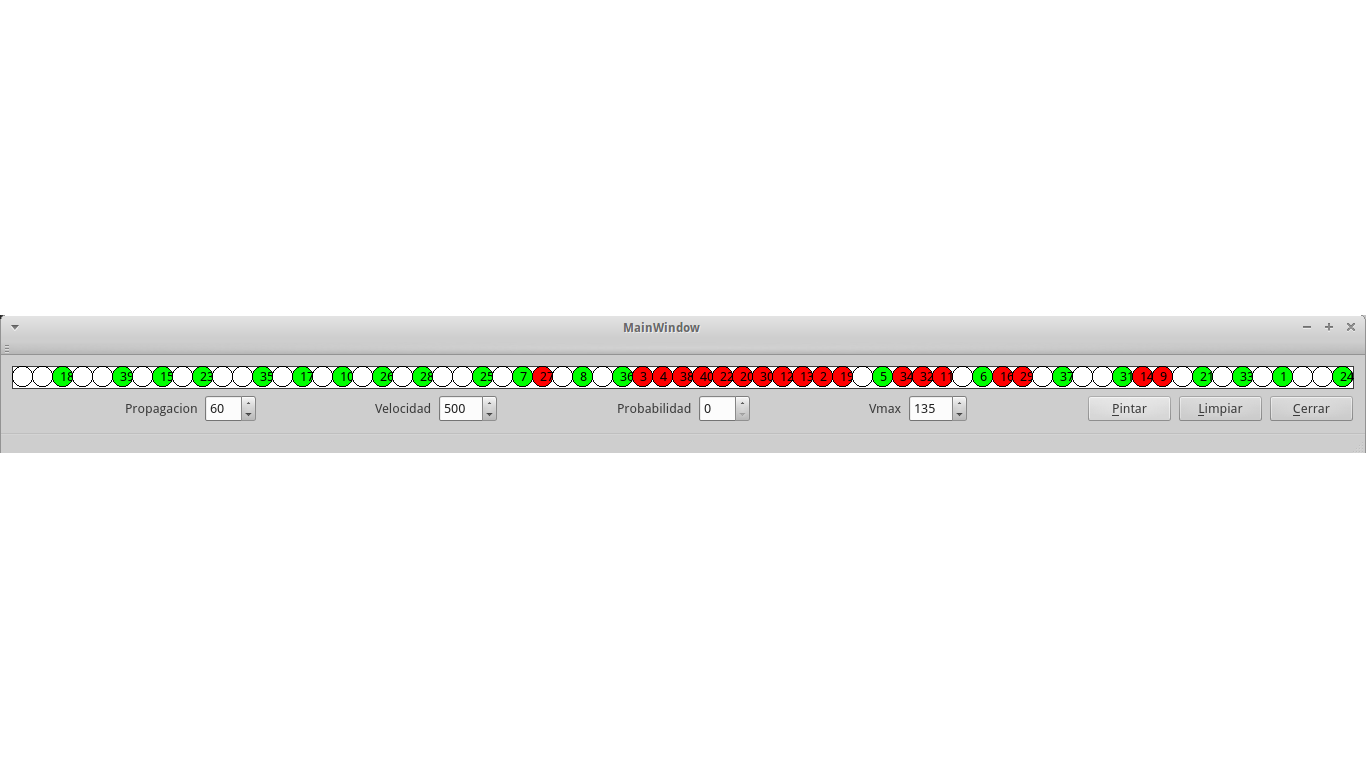
\includegraphics[width=15cm, height=7cm]{28}
\\
podemos ver que el comportamiento sin probabilidad es que los estancamientos se hacen mas grandes y se multiplican ahora tenemos 5 estancamientos por separado que no se juntan y permanecen a una distancia casi constante.
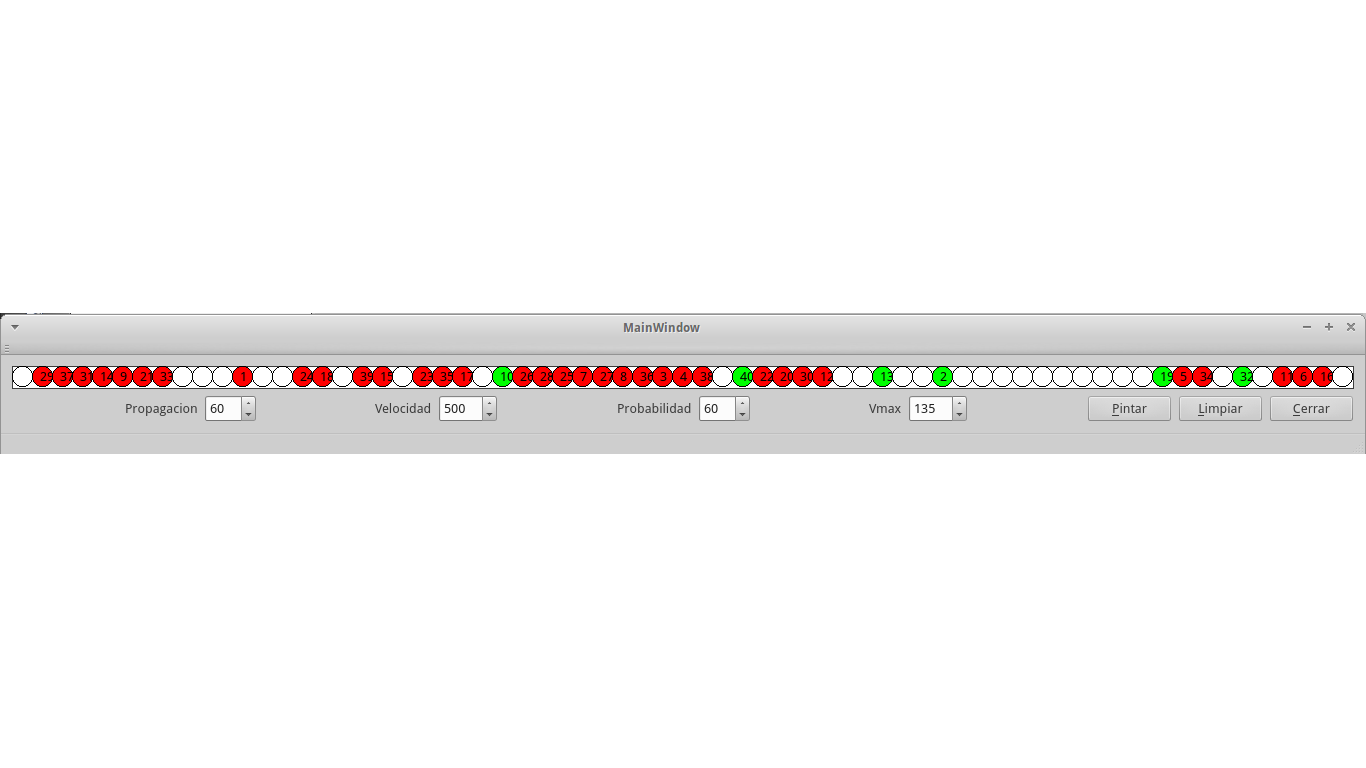
\includegraphics[width=15cm, height=7cm]{29}
\\
con probabilidad el sistema se satura de trafico y cae en uncaso similar a cuando llueve o cuando el trafico es mayor que el numero de carros que soporta la carretera.
\subsection{Prueba 9}
Densidad 70\% Vmax 135km/h probabilidad 0\%
\\
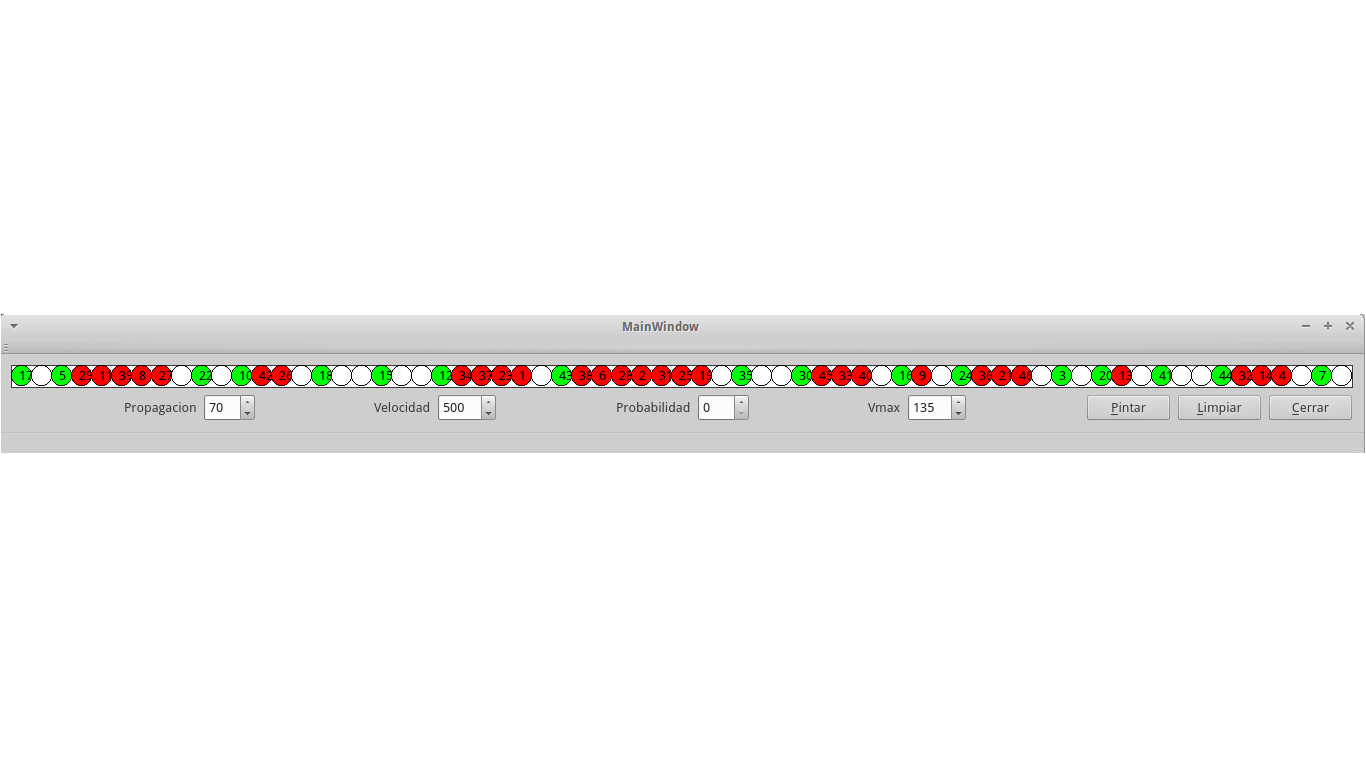
\includegraphics[width=15cm, height=7cm]{30}
\\
Con la densidad de 70\% podemos ver que el trafico se hace homogeneo se aprecia que ya existen saturaciones similares al trafico en hora pico.
\\
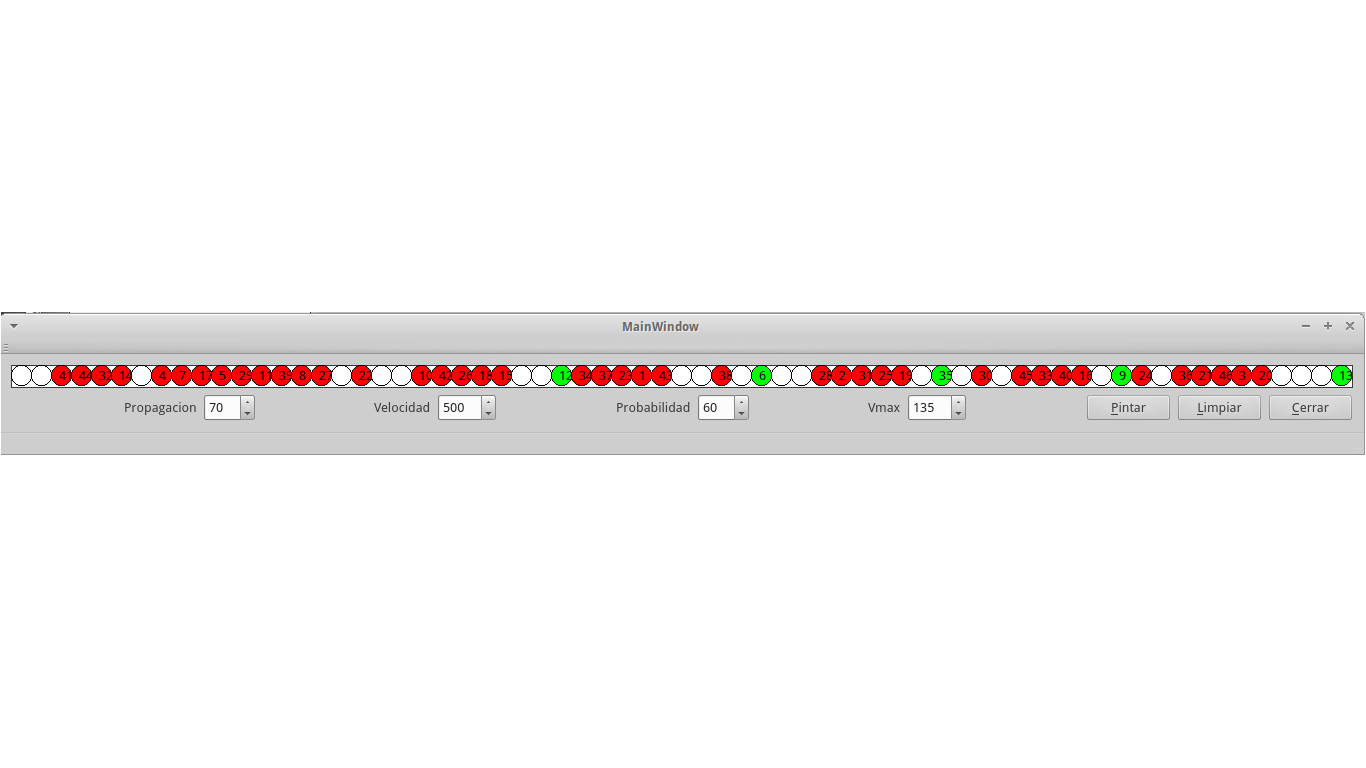
\includegraphics[width=15cm, height=7cm]{31}
\\
Si le agregamos la probabilidad podemos ver el caso del famoso trafico parado que se puede dar cuando en hora pico se agrega algun factor como lluvia, o que se descomponga algun carro.
\section{Pruebas Multilinea}

Veremos un ejemplo de lo mismo pero con lieas cruzadas veremos comportamientos muy similares pero al tener mas agentes el comportamiento se ve mas caotico.
\subsection{Prueba 1}
Densidad 10\% Vmax 135km/h probabilidad 0\%
\\

\includegraphics[width=15cm, height=7cm]{32}
\\
Es una distribucion de carros separada en la que no se puede ver trafico en ninguna parte por que existe un separacion considerable de carro a carro.
agregando probabilidad vemos lo siguiente.
\\
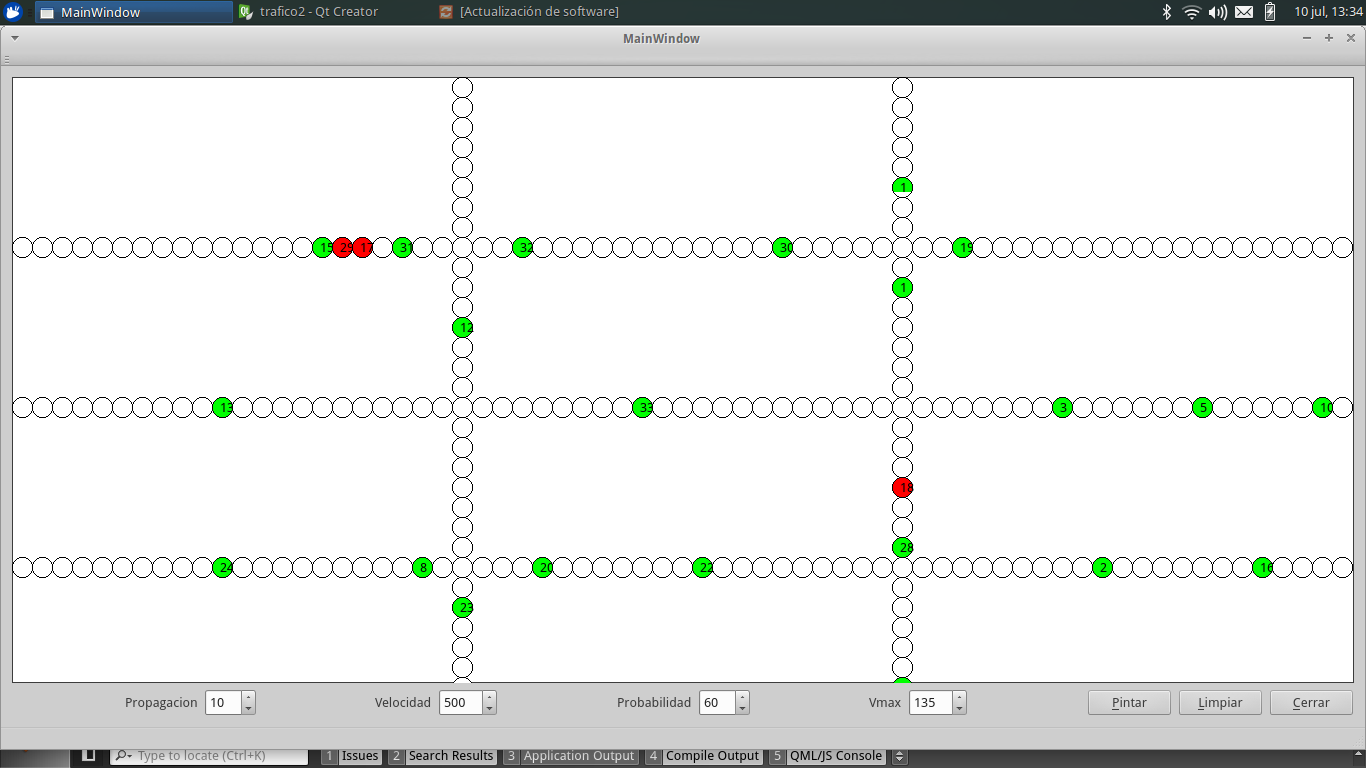
\includegraphics[width=15cm, height=7cm]{33}
\\
Se llegan a formar atorones muy pequeños que tienden a desaparecer con el tiempo.
\subsection{Prueba 2}
Densidad 30\% Vmax 135km/h probabilidad 0\%
\\
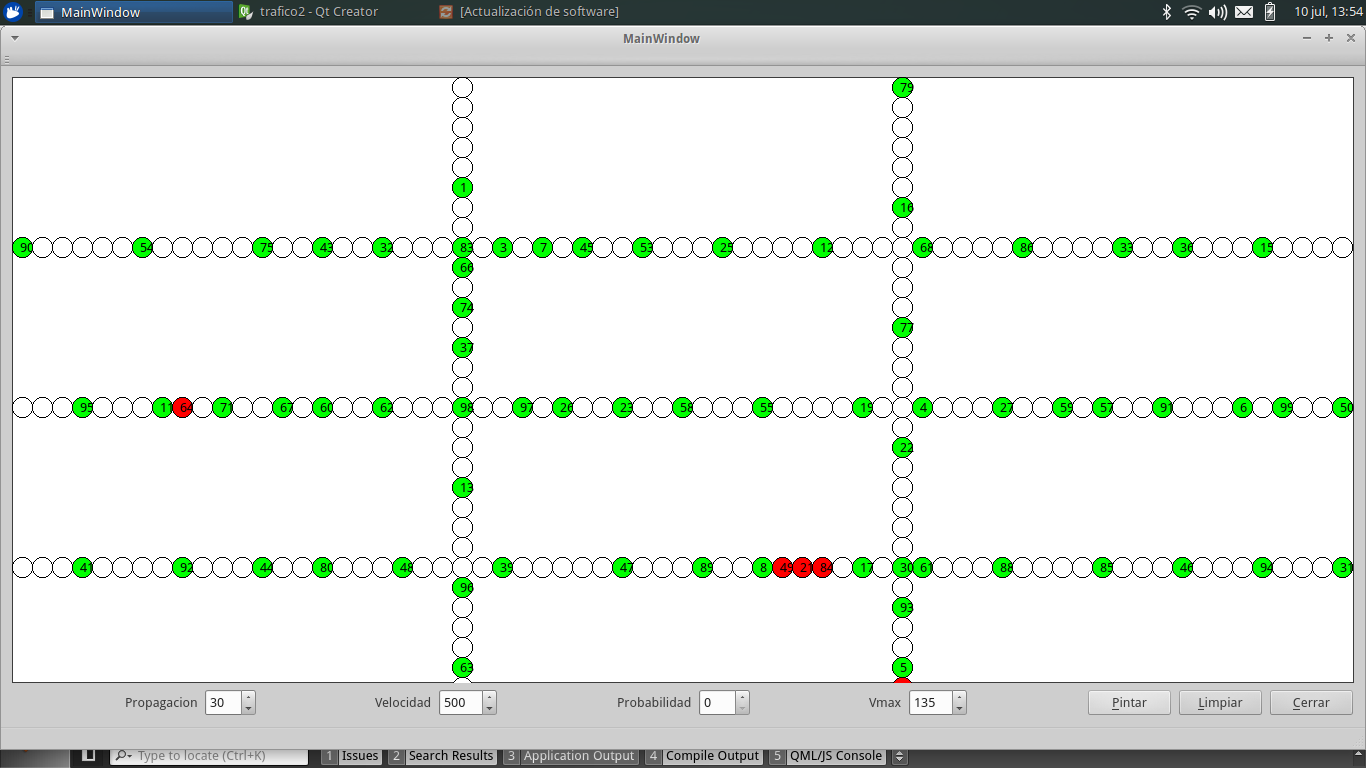
\includegraphics[width=15cm, height=7cm]{34}
\\
se pueden ver ya sturaciones desde el inicio del sistema que no desaparecen si no que giran en el sistema este es el caso que vimos en la simulacion de una sola linea donde la gente se cruza las calles cuando no deben.
\\
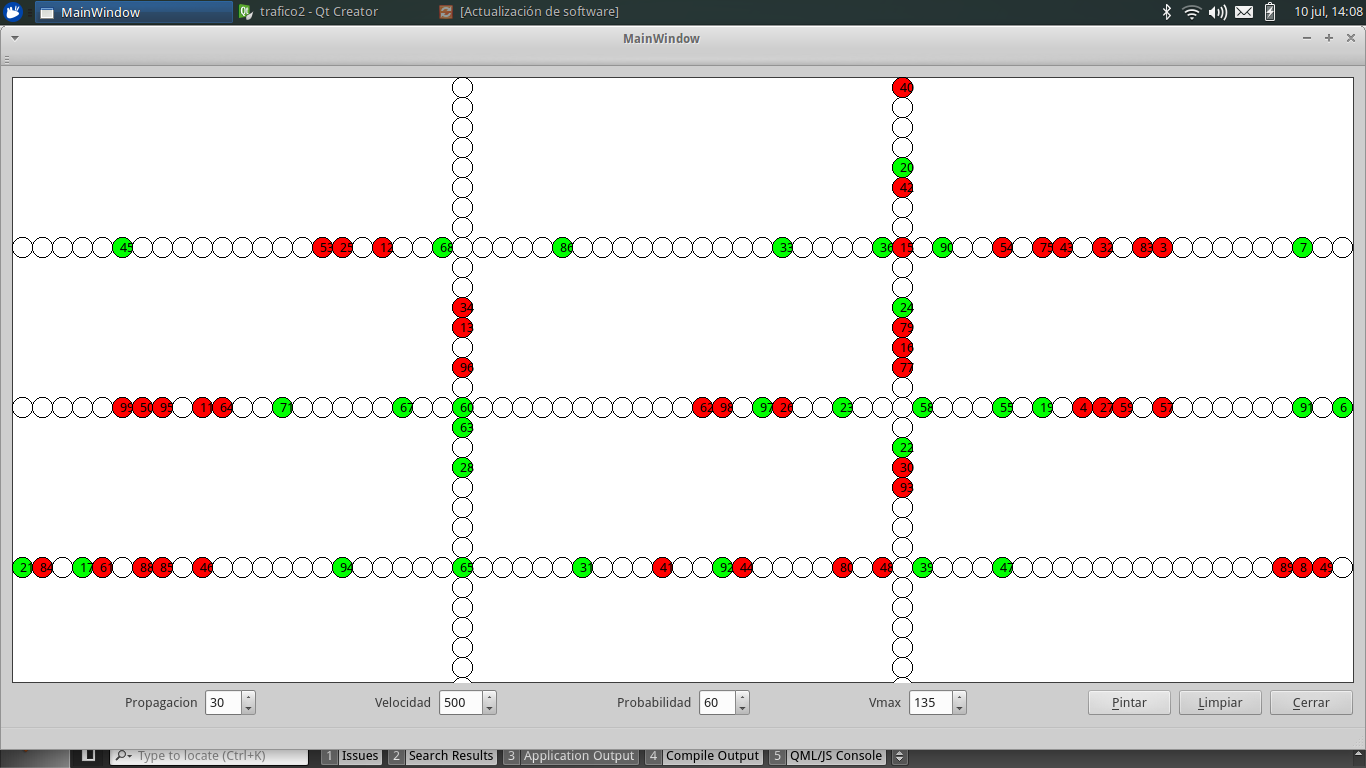
\includegraphics[width=15cm, height=7cm]{35}
\\
Se va que ya tenemos trafico mas abundante al momento de agregarle probabilidad, se crea algo de caos pero aun asi se ve que los carros continuan su camino.
\subsection{Prueba 3}
Densidad 70\% vmax 135km/h probabilidad 0\%
\\
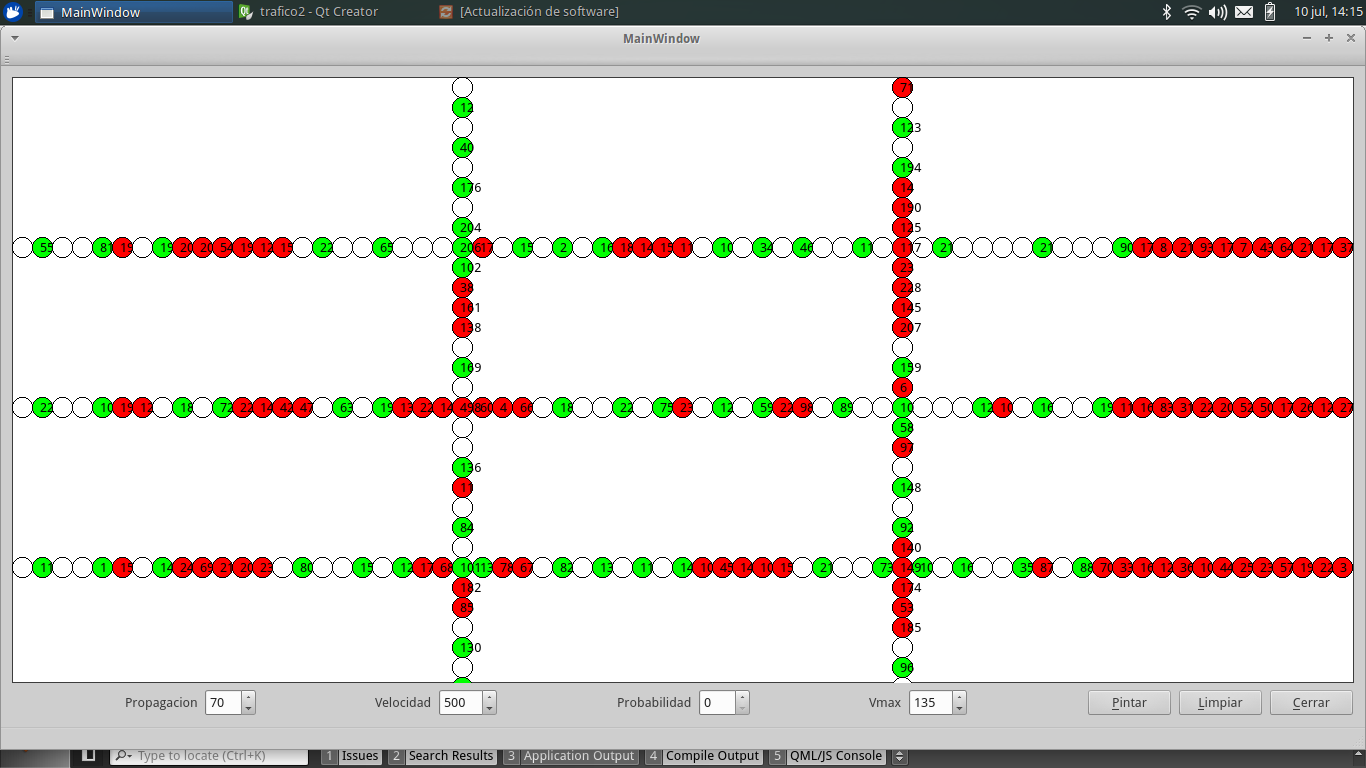
\includegraphics[width=15cm, height=7cm]{36}
\\
En este caso ya tenemos un trafico amplio que se ve pero aun no es trafico parado este caso de trafico parado si lo podemos ver en el caso con probabilidad.
\\
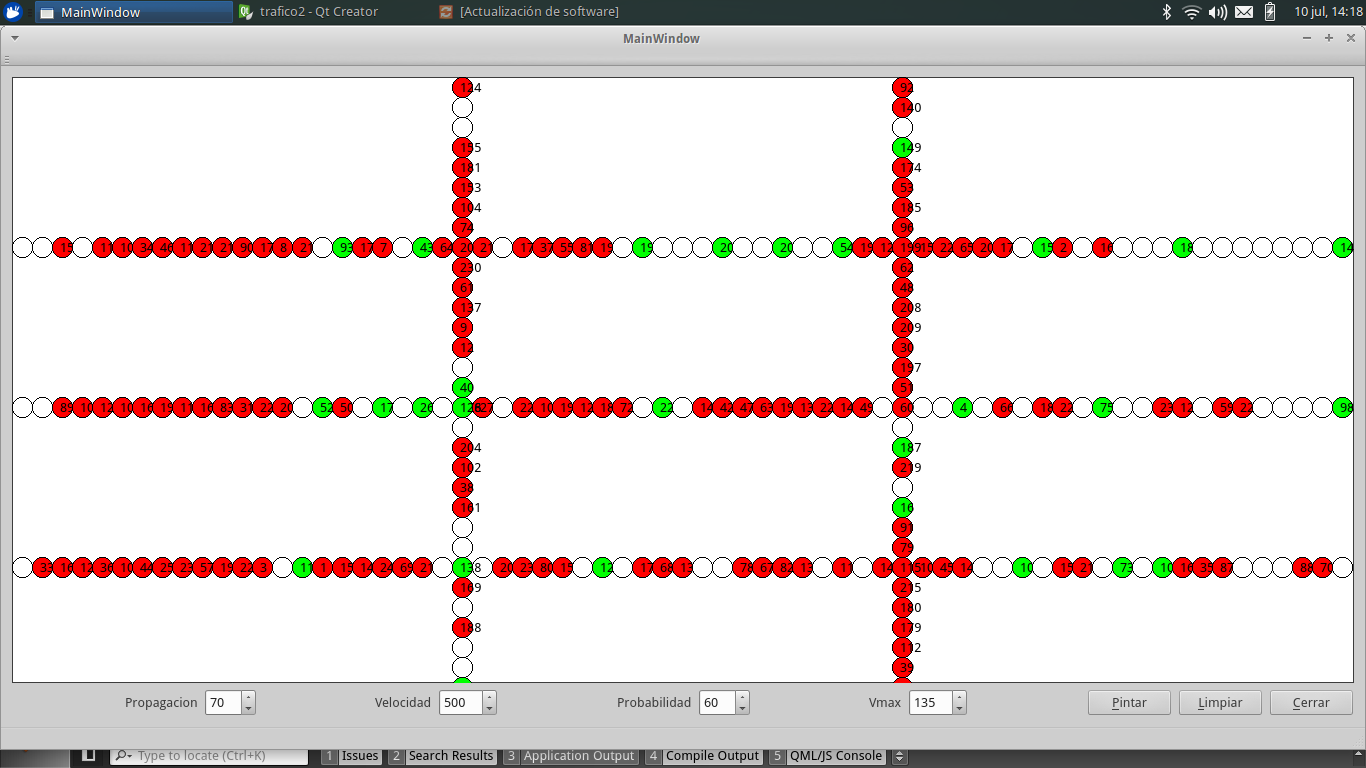
\includegraphics[width=15cm, height=7cm]{37}
\\
\end{document}
